%%%%%%%%%%%%%%%%%%%%%%%%%%%%%%%%%%%%%%%%%
% kaobook
% LaTeX Template
% Version 1.2 (4/1/2020)
%
% This template originates from:
% https://www.LaTeXTemplates.com
%
% For the latest template development version and to make contributions:
% https://github.com/fmarotta/kaobook
%
% Authors:
% Federico Marotta (federicomarotta@mail.com)
% Based on the doctoral thesis of Ken Arroyo Ohori (https://3d.bk.tudelft.nl/ken/en)
% and on the Tufte-LaTeX class.
% Modified for LaTeX Templates by Vel (vel@latextemplates.com)
%
% License:
% CC0 1.0 Universal (see included MANIFEST.md file)
%
%%%%%%%%%%%%%%%%%%%%%%%%%%%%%%%%%%%%%%%%%

\documentclass[
	fontsize=10pt, % Base font size
	twoside=false, % Use different layouts for even and odd pages (in particular, if twoside=true, the margin column will be always on the outside)
	%open=any, % If twoside=true, uncomment this to force new chapters to start on any page, not only on right (odd) pages
	%chapterprefix=true, % Uncomment to use the word "Chapter" before chapter numbers everywhere they appear
	%chapterentrydots=true, % Uncomment to output dots from the chapter name to the page number in the table of contents
	numbers=noenddot, % Comment to output dots after chapter numbers; the most common values for this option are: enddot, noenddot and auto (see the KOMAScript documentation for an in-depth explanation)
	%draft=true, % If uncommented, rulers will be added in the header and footer
	%overfullrule=true, % If uncommented, overly long lines will be marked by a black box; useful for correcting spacing problems
]{kaobook}

\newenvironment{diag}
{
	\begin{center}
	\begin{tikzcd}
	}
	% Diagrama
	{
	\end{tikzcd}
	\end{center}
}

%________________________ Gráficos _______________________________
%\usepackage[dvips]{graphicx}	%Gráficos externos	
%\usepackage{tikz-cd}			%Diagramas conmutativos
%\usepackage{tikz,pgfplots}		%Imágenes en tikz

%________________________ Símbolos especiales ___________________
%\usepackage{amsmath,amsthm,amssymb}	%Sociedad americana
%\usepackage{mathtools,mathrsfs}			%Fuentes para math mode

%________________________ Hipervínculos _________________________
%\usepackage{url}				%Externo
%\usepackage[section]{placeins}	%Sección
%\usepackage{hyperref}			%Referencia

%________________________ Tablas _______________________________
%\usepackage{subcaption}	%Subcaption
%\usepackage{showlabels}	%Mostrar etiquetas
%\usepackage{appendix}	%Apéndices
%_____Topología________________________________________________________________
\DeclareMathOperator{\con}{con}		%Envoltura convexa
\DeclareMathOperator{\id}{id}		%Identidad
\DeclareMathOperator{\cte}{Cte}		%Aplicación constante
\newcommand{\p}{\partial}			%Operador borde


%_____Álgebra lineal___________________________________________________________
\DeclareMathOperator{\Gl}{Gl}				%Grupo lineal
\DeclareMathOperator{\End}{End}				%Grupo de endomorfismos
\DeclareMathOperator{\rk}{rk}				%Rango
\DeclareMathOperator{\im}{Im}				%Imagen
\newcommand{\m}[2]{\mathcal{M}_{#1}(#2)}	%Anillo de matrices
\newcommand{\la}{\left\langle}				%Antilambda izquierda
\newcommand{\ra}{\right\rangle}				%Antilambda derecha
\DeclareMathOperator{\sgn}{sgn}				%Signatura
\DeclareMathOperator{\ord}{ord}				%Orden

%____Tipografías_______________________________________________________________
\newcommand{\mb}[1]{\mathbb{#1}}		%Blackboard
\newcommand{\mc}[1]{\mathcal{#1}}		%Calligraphic
\newcommand{\ms}[1]{\mathscr{#1}}		%Script
\newcommand{\mf}[1]{\mathfrak{#1}}		%Fraktur
\newcommand{\bs}[1]{\boldsymbol{#1}}	%Bold
\newcommand{\eps}{\varepsilon}			%Épsilon

%_____Letra ш__________________________________________________________________
\DeclareFontFamily{U}{wncy}{}
\DeclareFontShape{U}{wncy}{m}{n}{<->wncyr10}{}
\DeclareSymbolFont{mcy}{U}{wncy}{m}{n}
\DeclareMathSymbol{\Sh}{\mathord}{mcy}{"58}

%_____Escribir encima de un símbolo_____________________________________________
\newcommand{\arriba}[2]{\stackrel{\mathclap{#1}}{#2}}


\begin{document}

%----------------------------------------------------------------------------------------
%	BOOK INFORMATION
%----------------------------------------------------------------------------------------

\titlehead{Homología singular}
\subject{Use this document as a template}

\title[Teoría de homología singular]{Teoría de homología singular}
\subtitle{Introducción a los espacios CW-complejos}

\author[Hannah Muñoz Cabello]{Hannah Muñoz Cabello}

\date{\today}

%\publishers{An Awesome Publisher}

%----------------------------------------------------------------------------------------

\frontmatter % Denotes the start of the pre-document content, uses roman numerals

%----------------------------------------------------------------------------------------
%	OPENING PAGE
%----------------------------------------------------------------------------------------

%\makeatletter
%\extratitle{
%	% In the title page, the title is vspaced by 9.5\baselineskip
%	\vspace*{9\baselineskip}
%	\vspace*{\parskip}
%	\begin{center}
%		% In the title page, \huge is set after the komafont for title
%		\usekomafont{title}\huge\@title
%	\end{center}
%}
%\makeatother

%----------------------------------------------------------------------------------------
%	COPYRIGHT PAGE
%----------------------------------------------------------------------------------------


\begingroup % Local scope for the following commands

% Define the style for the TOC, LOF, and LOT
%\setstretch{1} % Uncomment to modify line spacing in the ToC
%\hypersetup{linkcolor=blue} % Uncomment to set the colour of links in the ToC
\setlength{\textheight}{23cm} % Manually adjust the height of the ToC pages

% Turn on compatibility mode for the etoc package
\etocstandarddisplaystyle % "toc display" as if etoc was not loaded
\etocstandardlines % toc lines as if etoc was not loaded

\tableofcontents % Output the table of contents

\listoffigures % Output the list of figures

% Comment both of the following lines to have the LOF and the LOT on different pages
\let\cleardoublepage\bigskip
\let\clearpage\bigskip

\listoftables % Output the list of tables

\endgroup

%----------------------------------------------------------------------------------------
%	DEDICATION
%----------------------------------------------------------------------------------------

\dedication{
	The harmony of the world is made manifest in Form and Number, and the heart and soul and all the poetry of Natural Philosophy are embodied in the concept of mathematical beauty.\\
	\flushright -- D'Arcy Wentworth Thompson
}

%----------------------------------------------------------------------------------------
%	OUTPUT TITLE PAGE AND PREVIOUS
%----------------------------------------------------------------------------------------

% Note that \maketitle outputs the pages before here

% If twoside=false, \uppertitleback and \lowertitleback are not printed
% To overcome this issue, we set twoside=semi just before printing the title pages, and set it back to false just after the title pages
\KOMAoptions{twoside=semi}
\maketitle
\KOMAoptions{twoside=false}

%----------------------------------------------------------------------------------------
%	PREFACE
%----------------------------------------------------------------------------------------

%\chapter*{Preface}
\addcontentsline{toc}{chapter}{Preface} % Add the preface to the table of contents as a chapter

I am of the opinion that every \LaTeX\xspace geek, at least once during 
his life, feels the need to create his or her own class: this is what 
happened to me and here is the result, which, however, should be seen as 
a work still in progress. Actually, this class is not completely 
original, but it is a blend of all the best ideas that I have found in a 
number of guides, tutorials, blogs and tex.stackexchange.com posts. In 
particular, the main ideas come from two sources:

\begin{itemize}
	\item \href{https://3d.bk.tudelft.nl/ken/en/}{Ken Arroyo Ohori}'s 
	\href{https://3d.bk.tudelft.nl/ken/en/nl/ken/en/2016/04/17/a-1.5-column-layout-in-latex.html}{Doctoral 
	Thesis}, which served, with the author's permission, as a backbone 
	for the implementation of this class;
	\item The 
		\href{https://github.com/Tufte-LaTeX/tufte-latex}{Tufte-Latex 
			Class}, which was a model for the style.
\end{itemize}

The first chapter of this book is introductive and covers the most 
essential features of the class. Next, there is a bunch of chapters 
devoted to all the commands and environments that you may use in writing 
a book; in particular, it will be explained how to add notes, figures 
and tables, and references. The second part deals with the page layout 
and design, as well as additional features like coloured boxes and 
theorem environments.

I started writing this class as an experiment, and as such it should be 
regarded. Since it has always been indended for my personal use, it may 
not be perfect but I find it quite satisfactory for the use I want to 
make of it. I share this work in the hope that someone might find here 
the inspiration for writing his or her own class.

\begin{flushright}
	\textit{Federico Marotta}
\end{flushright}


%----------------------------------------------------------------------------------------
%	TABLE OF CONTENTS & LIST OF FIGURES/TABLES
%----------------------------------------------------------------------------------------


\begingroup % Local scope for the following commands

% Define the style for the TOC, LOF, and LOT
%\setstretch{1} % Uncomment to modify line spacing in the ToC
%\hypersetup{linkcolor=blue} % Uncomment to set the colour of links in the ToC
\setlength{\textheight}{23cm} % Manually adjust the height of the ToC pages

% Turn on compatibility mode for the etoc package
\etocstandarddisplaystyle % "toc display" as if etoc was not loaded
\etocstandardlines % toc lines as if etoc was not loaded

\tableofcontents % Output the table of contents

\listoffigures % Output the list of figures

% Comment both of the following lines to have the LOF and the LOT on different pages
\let\cleardoublepage\bigskip
\let\clearpage\bigskip

\listoftables % Output the list of tables

\endgroup

%----------------------------------------------------------------------------------------
%	MAIN BODY
%----------------------------------------------------------------------------------------

\mainmatter % Denotes the start of the main document content, resets page numbering and uses arabic numbers
\setchapterstyle{kao} % Choose the default chapter heading style

\input{capitulos/introduccion.tex}
\setchapterpreamble[u]{\margintoc}

\chapter{Grupos de homología singular}
\section{Símplices singulares}
Decimos que una familia de puntos $S=\{x_0, \dots, x_p\} \subset \mb{R}^n$ es
\textbf{afínmente independiente} si, dados $\lambda_1,\dots,\lambda_n \in
\mb{R}$, $\mu_1,\dots,\mu_n \in \mb{R}$ tales que
\begin{align*}
\sum^p_{i=0}\lambda_ix_i=\sum^p_{i=0}\mu_ix_i;
&&
\sum^p_{i=0}\lambda_i=\sum^p_{i=0}\mu_i
\end {align*}
se verifica que $\lambda_i=\mu_i$ para todo $1\leq i \leq n$.

\begin{proposition}
La familia de puntos $S=\{x_0, \dots, x_p\} \subset \mb{R}^n$ es afínmente
independiente si y sólo si la familia de vectores
\[T=\{x_1-x_0,\dots,x_p-x_0\}\]
es linealmente independiente.
\end{proposition}

\begin{proof}
Supongamos que $S$ es afínmente independiente y sean $\lambda_1,\dots,
\lambda_p$ tales que
\begin{equation}
\labeq{CombLinNula}
\sum^p_{i=1}\lambda_i(x_i-x_0)=0 \iff
\sum^p_{i=1}\lambda_ix_i=x_0\sum^p_{i=1}\lambda_i
\end{equation}

Definimos $\lambda_0=-\lambda_1-\dots-\lambda_p$. Por construcción, se
verifica que $\lambda_0+\lambda_1+\dots+\lambda_p=\lambda_0-\lambda_0=0$.
Aplicando \eqref{CombLinNula},
\[0=\sum^p_{i=1}\lambda_i(x_i-x_0)=
\sum^p_{i=1}\lambda_i x_i-x_0\sum^p_{i=1}\lambda_i=
\sum^p_{i=0}\lambda_i x_i\]

Por otro lado, también podemos escribir $0=0x_0+\dots+0x_p$. Dado que $S$ es una
familia afínmente independiente, $\lambda_i=0$ para todo $i=1,\dots,n$.
Por tanto, $T$ es linealmente independiente.

Recíprocamente, sea $T$ una familia linealmente independiente y
$\mu_0,\dots,\mu_p \in \mb{R}$, $\alpha_0,\dots,\alpha_p \in \mb{R}$ tales que
\begin{align*}
\sum_{i=0}^p \mu_ix_i=\sum_{i=0}^p \alpha_ix_i;
&&
\sum_{i=0}^p \mu_i=\sum_{i=0}^p \alpha_i
\end{align*}
Combinando ambas igualdades, deducimos que
\begin{align*}
0=\sum^p_{i=0}(\mu_i-\alpha_i)x_i
	&=\sum^p_{i=0}(\mu_i-\alpha_i)x_i-0x_0=\\
	&=\sum^p_{i=0}(\mu_i-\alpha_i)x_i-
	\left(\sum^p_{i=0}(\mu_i-\alpha_i)\right)x_0=\\
	&=\sum^p_{i=1}(\mu_i-\alpha_i)(x_i-x_0)
\end{align*}

Dado que $T$ es linealmente independiente, se sigue que
\[\mu_i-\alpha_i=0 \iff \mu_i=\alpha_i \quad (i=1,\dots, p)\]

Sabiendo que la suma de todos los $\mu_i$ es la misma que la de todos los
$\alpha_i$, se sigue que $\mu_0=\alpha_0$. Por tanto, $S$ es afínmente
independiente.
\end{proof}

\begin{marginfigure}
\begin{tikzpicture}[scale=0.6]
%Puntos
\draw (3,3)[fill=black] circle (1pt);
\draw (3,3.5) node {$a$};

\draw (0,0)[fill=black] circle (1pt);
\draw (0,-.5) node {$b$};

\draw (-3,3)[fill=black] circle (1pt);
\draw (-3,3.5) node {$c$};

%Vectores
\draw[-to] (0,0) -- (1,1);
\draw[-to] (0,0) -- (-1,1);

%Líneas
\draw[dashed] (-1,-1) -- (4,4);
\draw (2,1.5) node {$L_1$};

\draw[dashed] (1,-1) -- (-4,4);
\draw (-2,1.5) node {$L_2$};
\end{tikzpicture}
\caption[Puntos afínmente independientes]{La independencia afín es una forma de definir independencia lineal
en conjuntos afines, donde los elementos son puntos y no vectores.}
\end{marginfigure}

\begin{remark}
Sea $S \subset \mb{R}^n$ un conjunto afínmente independiente y $(a,b,c)$ una
terna de elementos de $S$ con $a\neq b \neq c$. Si $S$ es afínmente
independiente, debe pasar que los vectores $a-b$ y $b-c$ sean linealmente
independientes.

Como $a-b\neq 0$, existe una recta afín $L_1 \subset \mb{R}^n$ que tiene a
$a-b$ como vector director. De la misma forma, existe otra recta afín
$L_2 \subset \mb{R}^n$ que tiene a $b-c$ como vector director. Por independencia
lineal, se tiene que $L_1$ no es paralelo a $L_2$, por lo que $a \not\in L_2$ y
$c \not\in L_1$.

Por tanto, un conjunto afínmente independiente es aquel en el que no hay tres
puntos colineales.
\end{remark}

\begin{definition}
Un \textbf{$p$-símplice} es la envoltura convexa de una familia de puntos $\{x_0,
\dots,x_p\} \subset \mb{R}^n$ afínmente independientes. Dichos puntos reciben el
nombre de \textbf{vértices} del símplice.
\end{definition}

\marginnote[-2.2cm]{
\begin{kaobox}[frametitle=Envoluta convexa]
Un $C \subseteq \mb{R}^n$ no vacío es convexo si, dados $x,y \in C$, $C$ contiene al segmento $[x,y]$.

Si $A \subset \mb{R}^n$ es no vacío, se define su envoltura convexa como el menor subconjunto convexo que contiene a $A$,
\[\con(A)=\bigcup_{x,y \in A}[x,y]\]
\end{kaobox}
}

\begin{remark}
\begin{enumerate}
\item Sea $A$ una familia de puntos afínmente independientes de $\mb{R}^n$ e
\[i\colon \mb{R}^n \hookrightarrow \mb{R}^m\]
la inclusión. Se tiene que $i(A)$ es una familia de puntos afínmente
independiente de $\mb{R}^m$, por lo que los símplices de $\mb{R}^n$ son también
símplices en $\mb{R}^m$.
\item Dado que los puntos que generan al símplice son afínmente independientes, debe
pasar que $n \geq p$. Por ello, se entiende que, si $S \subset \mb{R}^n$ es un
$p$-símplice, $p \leq n$.
\end{enumerate}
\end{remark}

\begin{proposition}\labprop{BaseVertices}
Sea $S\subset \mb{R}^n$ un $p$-símplice y $\{x_0,\dots x_p\}$ una familia
afínmente independiente de puntos contenidos en $S$. Dado un punto $x \in S$,
existe una familia única de escalares $t_0,\dots, t_p \in [0,1]$ tales que
\begin{align*}
x=\sum^p_{i=0}t_ix_i; && \sum^p_{i=0}t_i=1
\end{align*}
Por lo que una familia de vértices de un símplice es el equivalente a una base
en un espacio vectorial.
\end{proposition}

Decimos que un $p$-símplice está \textbf{ordenado} cuando se aplica una relación
de orden determinada sobre sus vértices.

\begin{ejem}
Sean $a=(1,0,0)$, $b=(0,1,0)$ y $c=(0,0,1)$. La envoltura convexa de $\{a,b,c\}$
es un 2-símplice, que denotaremos como $\sigma$. Si $e_1=a$, $e_2=b$ y $e_3=c$,
la relación de orden
\[e_i \leq e_j \iff i \leq j\]
hace que $\sigma$ sea un 2-símplice ordenado.
\end{ejem}

\begin{marginfigure}
\centering
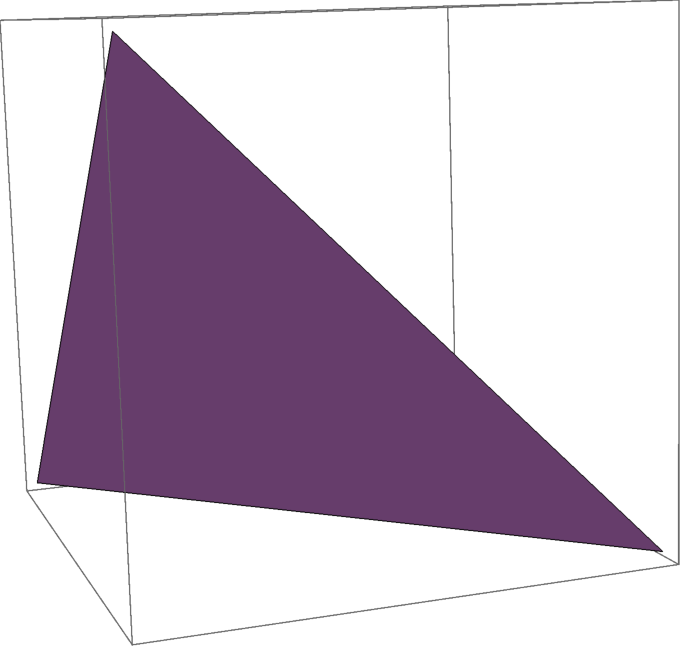
\includegraphics{Figures/2Simplice.pdf}
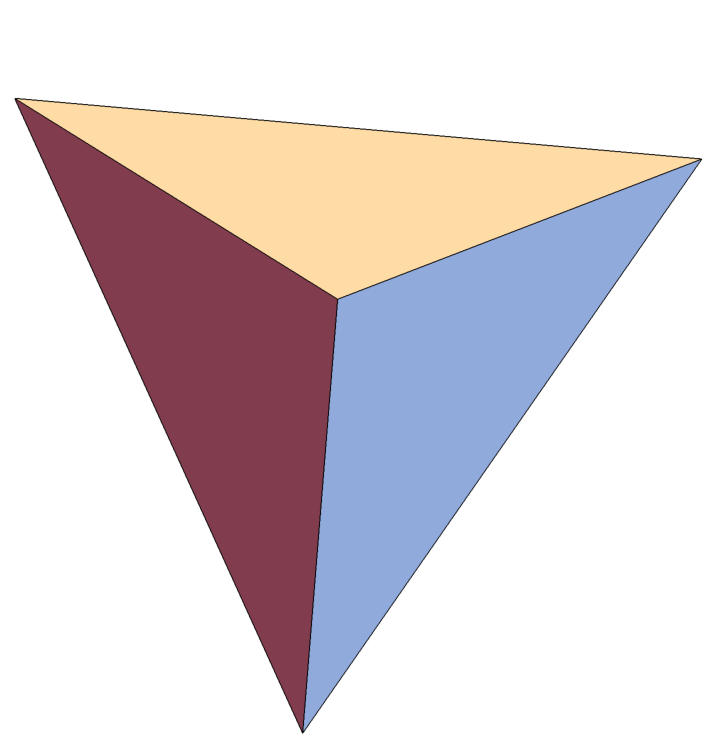
\includegraphics{Figures/Simplice.pdf}
\caption[Triángulo y tetraedro]{Los triángulos y tetraedros constituyen ejemplos de símplices. Podemos crear una teoría de homología utilizando sólo símplices, pero se limitaría a espacios topológicos contenidos en $\mb{R}^n$.}
\labfig{123Simplice}
\end{marginfigure}

\begin{nota}
Sea $\{e_1, \dots, e_{n+1}\}$ la base canónica de $\mb{R}^{n+1}$. La envoltura
convexa de los puntos $\{e_1, \dots, e_{n+1}\}$ es un $n$-símplice, que
denotaremos como $\sigma_n$. Por \refprop{BaseVertices}, los puntos
de $\sigma_n$ son de la forma
\begin{align*}
(t_1,\dots,t_{n+1}) \in \mb{R}^{n+1}; && t_1+\dots+t_{n+1}=1
\end{align*}

Sea $S=\{x_0,\dots,x_n\}\subset \mb{R}^m$ una familia de puntos afínmente
independientes: la aplicación continua
\begin{diag}
f\colon \sigma_n \arrow[r]                   & \con(S)            \\[-0.8cm]
{(t_0,\dots,t_n)} \arrow[r, maps to] & \displaystyle\sum^n_{i=0}t_ix_i
\end{diag}
establece una biyección entre $\sigma_n$ y $\con(S)$. Dado que $\sigma_n$ es
compacto y $\con(S)$ es un espacio de Hausdorff, $f$ es un homeomorfismo, por lo
que $\con(S)$ es homeomorfo a $\sigma_n$.
\end{nota}

De la observación anterior, se sigue que todo $p$-símplice de $\mb{R}^{p+1}$ es
homeomorfo a $\sigma_p$, por lo que podemos considerarlo como el representante
canónico de todos los $p$-símplices. En consecuencia, $\sigma_p$ recibe el
nombre de \textbf{$p$-símplice estándar}.

\begin{ejem}
\labexample{012simp}
\begin{enumerate}
\item El conjunto $\sigma_0$ es el singulete formado por el punto $1 \in \mb{R}$.
\item El conjunto $\sigma_1$ es el segmento que une los puntos $(1,0)$ y $(0,1)$
de $\mb{R}^2$.
\item El conjunto $\sigma_2$ es el triángulo de vértices $e_1, e_2, e_3 \in
\mb{R}^3$. 
\end{enumerate}
\end{ejem}

Si nos limitamos a subespacios topológicos en $\mb{R}^n$, podemos crear una
teoría de homología utilizando sólo símplices (\cite{Lujan18}). Sin embargo, si
queremos definir una teoría que cubra todos los espacios topológicos, necesitamos
transportar el símplice utilizando aplicaciones continuas.

\begin{definition}
Sea $X$ un espacio topológico. Un \textbf{$p$-símplice singular} de $X$ es una
aplicación continua
\[\phi\colon \sigma_p \to X\]
\end{definition}

\begin{ejem}\labexample{S1Complejo}
Sea $\mb{D}=\{z \in \mb{C}: |z|=1\}$. La aplicación
\begin{diag}
\phi\colon \sigma_1 \arrow[r]	& \mb{D}\\[-0.8cm]
(t_0,t_1) \arrow[maps to,r] 	& e^{\pi i t_0}
\end{diag}
es un símplice singular, que envía al 1-símplice estándar en la mitad superior
del 1-símplice mostrado en \reffig{Circunferencia}.

$\phi(\sigma_1)$ no es un segmento desde el punto de vista geométrico porque
tiene curvatura no nula, pero sí lo es desde un punto de vista topológico,
ya que $\phi$ es un homeomorfismo y $\sigma_1$ es un segmento.
\end{ejem}

\begin{marginfigure}[ht]
\begin{tikzpicture}
\draw [to-to] (-2.5,0) -- (2.5,0);
\draw [to-to] (0,-2.5) -- (0,2.5);

\draw[thick,dashed] (0,0) circle (2cm);

\draw[thick] (2,0) arc (0:180:2);
\draw (1,2.2) node {$\phi(\sigma_1)$};
\end{tikzpicture}
\caption[Circunferencia]{La curva $\phi(\sigma_1)$ dada por el símplice singular $\phi$ de \refexample{S1Complejo}. Los símplices singulares amoldan el símplice
estándar al espacio de llegada usando su continuidad.}
\labfig{Circunferencia}
\end{marginfigure}

Dado un $p \in X$ y un espacio topológico $Y$, toda aplicación constante
$\cte_p\colon Y \to X$ se identifica con el 0-símplice singular
$\phi_p\colon \sigma_0 \to X$ que envía al punto 1 en $p$. De la
misma forma, si $I$ es un intervalo cerrado de $\mb{R}$, todo camino
$\alpha\colon I \to X$ se identifica con el 1-símplice singular
\begin{diag}
\psi\colon	\sigma_1 \arrow[r]             & X            \\[-0.8cm]
		{(t_0,t_1)} \arrow[r, maps to] & \alpha(t_0)
\end{diag}

Sean $X$, $Y$ espacios topológicos. Dada una aplicación continua $f\colon X
\to Y$ y un $p$-símplice singular $\phi\colon \sigma_p
\to X$, la aplicación
\[f_\#(\phi):=f\circ \phi\colon \sigma_p \to Y\]
es un $p$-símplice singular en $Y$ por ser composición de aplicaciones continuas.
Esto hace que toda aplicación continua dé lugar a una aplicación que envía
$p$-símplices singulares de $X$ en $p$-símplices singulares de $Y$.

\begin{proposition}\labprop{ComposicionAlmohadilla}
\begin{enumerate}
\item Si $\id_X$ es la aplicación identidad, $(\id_X)_\#$ también es la
aplicación identidad.
\item Si $f\colon X \to Y$ y $g\colon Y \to Z$ son
aplicaciones continuas,
\[(g\circ f)_\#=g_\#\circ f_\#\]
\end{enumerate}
\end{proposition}

Sea $X$ un espacio topológico, $\phi\colon \sigma_p \to X$ un
$p$-símplice singular y $0 \leq i \leq p$. Se define la \textbf{cara $i$-ésima
de $\phi$} como el $(p-1)$-símplice singular
\begin{diag}
\p_{(i)}\phi\colon \sigma_{p-1} \arrow[r] & X \\[-0.8cm]
{(t_0,\dots,t_{p-1})} \arrow[r, maps to] &
\phi(t_0,\dots,t_{i-1},0,t_{i},\dots,t_{p-1})
\end{diag}

\begin{ejem}
Considérese el 2-símplice singular
\begin{diag}
\phi\colon  \sigma_2 \arrow[r] & \mb{R}^3 \\[-0.8cm]
(x,y,z) \arrow[r, maps to] & (2x+2,2y+2,2z+2)
\end{diag}

Las caras de $\phi$ son los $1$-símplices singulares
\begin{align*}
\p_{(0)}\phi(u,v)=\phi(0,u,v)=(2,2u+2,2v+2)\\
\p_{(1)}\phi(u,v)=\phi(u,0,v)=(2u+2,2,2v+2)\\
\p_{(2)}\phi(u,v)=\phi(u,v,0)=(2u+2,2v+2,2)
\end{align*}

Desde un punto de vista geométrico, $\p_{(i)}\phi(\sigma_1)$ son las caras del
tetraedro $\phi(\sigma_2)$ para $i=0,1,2$.
\end{ejem}

\section{Grupos libres}
Sea $G$ un grupo abeliano y $n \in \mb{Z}$ un entero no nulo. Dado un $g \in G$,
se define el producto $ng$ como
\begin{align*}
ng:=\sum^n_{j=0}g	&& ng:=\sum^{-n}_{j=0}-g\\
(n>0)				&& (n < 0)
\end{align*}
Si $n=0$, se considera que $0g=0$ para todo $g \in G$.

Decimos que un subconjunto $S \subset G$ es un \textbf{sistema generador} de $G$
si, dado un $g \in G$, podemos hallar $b_1,\dots,b_n \in S$ y enteros
$\mu_1,\dots,\mu_n$ tales que
\[g=\mu_1b_1+\mu_2b_2+\dots+\mu_nb_n\]

\begin{definition}
Sea $G$ un grupo abeliano. Un sistema generador $B$ de $G$ es una \textbf{base}
si, dados $b_1,\dots,b_n \in B$ y enteros $\lambda_1,\dots,\lambda_n$,
\begin{align}
\labeq{SisLibre} \sum^n_{i=1}\lambda_ib_i=0 \implies \lambda_i=0
\end{align}
Decimos que $G$ es un \textbf{grupo libre} si admite una base.
\end{definition}

\begin{example}
Supongamos que $\mb{Q}^+=(\mb{Q},+)$ es un grupo libre generado por un cierto
conjunto $B \subseteq \mb{Q}$. Dados $\frac{a}{b}, \frac{c}{d} \in B$, se tiene
que
\[cb\frac{a}{b}-ad\frac{c}{d}=0\]
por lo que $B$ está formado por un único elemento.

Sea $p$ un número primo coprimo con $b$. Por ser $\mb{Q}^+$ libre, existirá un
entero $\alpha$ tal que
\[\frac{1}{p}=\alpha\frac{a}{b}\]
pero esto implica que $b=\alpha pa$, en contradicción con la premisa de que $p$
es coprimo con $b$. Por tanto, $\mb{Q}^+$ no es un grupo libre.
\end{example}

\subsection{Grupo libre generado por un conjunto}
\begin{proposition}
Sea $A \neq\emptyset$. Se define el grupo libre generado por $A$ como la familia
$\mc{F}(A)$ de todas las aplicaciones $f\colon A \to \mb{Z}$ que se
hacen cero casi por todas partes. Entonces, $\mc{F}(A)$ es un grupo libre dotado
con la suma elemento a elemento.
\end{proposition}

\marginnote[-2.2cm]{
\begin{kaobox}[frametitle=Aplicaciones nulas casi por todas partes]
Sea $A$ un conjunto no vacío. Decimos que una aplicación $f\colon A
\to \mb{Z}$ es \textbf{nula casi por todas partes} si podemos hallar un subconjunto $B \subseteq A$ finito tal que $f(x)=0$ para todo $x \in A\backslash B$.
\end{kaobox}
}

\begin{proof}
Dado un $a \in A$, se define $\mc{X}_a\colon A \to \mb{Z}$ como
\[\mc{X}_a(x)=\begin{cases}
1&\mbox{ si }x=a\\
0&\mbox{ si }x\neq a
\end{cases}\]
Notar que $\mc{X}_a$ es una aplicación nula casi por todas partes, por lo que
$\mc{X}_a \in \mc{F}(A)$. La base de $\mc{F}(A)$ será el conjunto
\[X:=\{\mc{X}_a: a\in A\} \subseteq \mc{F}(A)\]

Dada una aplicación $f \in \mc{F}(A)$, se define $\tilde{f}$ como
\[\tilde{f}=\sum_{a \in A}f(a)\mc{X}_a\]
Dado un $x \in A$,
\begin{equation}
\labeq{tildef}\tilde{f}(x)=\sum_{a \in A} f(a)\mc{X}_a(x)=
f(x)\underbrace{\mc{X}_x(x)}_{=1}+
\sum_{a \neq x}f(a)\underbrace{\mc{X}_a(x)}_{=0}=f(x)
\end{equation}
por lo que $\tilde{f}=f$. Por tanto, toda aplicación de $\mc{F}(A)$ es
combinación lineal de elementos de $X$, de forma que $X$ es un sistema generador
de $\mc{F}(A)$.

Sean $\mu_1,\dots,\mu_n$ enteros y $a_1,\dots,a_n \in A$ tales que
$\mu_1\mc{X}_{a_1}+\dots+\mu_n\mc{X}_{a_n}=0$. Dado un $1 \leq j \leq n$,
\[0=\sum^n_{i=1}\mu_i\mc{X}_{a_i}(a_j)=
\mu_j\underbrace{\mc{X}_{a_j}(a_j)}_{=1}+
\sum^n_{i \neq j}\mu_i\underbrace{\mc{X}_{a_i}(a_j)}_{=0}=\mu_j\]
por lo que $\mu_1,\dots,\mu_n=0$. Por tanto, $X$ es una base.
\end{proof}

Por convenio, se considera que $\{0\}=\mc{F}(\emptyset)$.

\begin{ejem}
$\mc{F}(\mb{N})$ es el conjunto de todas las sucesiones $(a_n)_{n=1}^\infty$
de $\mb{Z}$ con $a_n=0$ para casi todo $n \in \mb{N}$. Es decir, el anillo de
polinomios sobre $\mb{Z}$.
\end{ejem}

Notar que, si $A=\{a_1,\dots,a_n\}$, la aplicación
\begin{diag}
\Psi\colon \mc{F}(A) \arrow[r]	& \mb{Z}^n\\[-0.8cm]
f \arrow[maps to,r]			& (f(a_1),\dots,f(a_n))
\end{diag}
es un isomorfismo de grupos.

\section{Complejos de cadenas}
\begin{definition}
Un \textbf{grupo graduado} es una colección de grupos $G=\{G_n: n \in \mb{Z}\}$.
Diremos que $G$ es \textbf{abeliano} si todos los grupos $G_n$ lo son.
\end{definition}

Sean $G,H$ grupos graduados. Un \textbf{homomorfismo graduado} $f\colon G
\rightarrow H$ es una colección de homomorfismos
\[f_i\colon G_i \to H_{i+r} \quad (i \in \mb{Z})\]
siendo $r \in \mb{Z}$ un valor común para todos los $f_i$. Dicho entero se
denomina \textbf{grado} de $f$.

\begin{definition}
Dos grupos graduados $G$, $H$ son \textbf{isomorfos} si, dado un entero $p$,
existe un isomorfismo $f_p\colon G_p \to H_p$. Al homomorfismo
graduado $f=\{f_p\}_{p \in \mb{Z}}$ se le denomina \textbf{isomorfismo graudado}.
\end{definition}

\marginnote[-2.2cm]{
\begin{kaobox}[frametitle=Subgrupo normal]
Un subgrupo $H \leq G$ es normal si, dados $g \in G$ y $n \in N$, $ng=gm$ para algún $m \in N$. Esta condición es importante para poder garantizar que las clases del espacio cociente están bien definidas, pero se puede obviar cuando $G$ es abeliano.
\end{kaobox}
}

Si $G, H$ son grupos graduados, decimos que $H$ es un \textbf{subgrupo graduado}
de $G$ si, dado un entero $n$, $H_n \leq G_n$. En particular, si
$H_n$ es un subgrupo normal para todo $n$, se define el \textbf{grupo graduado
cociente} como
\[\frac{G}{H}:=\left\{\frac{G_i}{H_i}: i \in \mb{Z}\right\}\]

\begin{definition}
Un \textbf{complejo de cadenas} es un par de la forma $(G,\p)$, siendo $G$ un grupo graduado y $\p$ un endomorfismo de grado -1 tal que
\[\im  \p_n \leq \ker \p_{n-1}\]
La aplicación $\p$ recibe el nombre de \textbf{operador borde}.
\end{definition}

Diremos que un complejo de cadenas $(C,d)$ es \textbf{abeliano} si lo es $C$.

\begin{definition}
Sean $(C,d)$ y $(C',d')$ dos complejos de cadenas. Una \textbf{aplicación de
cadenas} es un homomorfismo graduado $\Phi\colon C \to C'$ de grado
$0$ tal que el siguiente diagrama es conmutativo para todo $n$:
\begin{diag}
C_{n+1} \arrow{r}{d_{n+1}} \arrow{d}{\Phi_{n+1}} & C_n \arrow{d}{\Phi_n} \\
C'_{n+1} \arrow{r}{d'_{n+1}}                     & C'_n                   
\end{diag}
\end{definition}

\subsection{Grupo de homología asociado a un complejo de cadenas}
Sea $(C,d)$ un complejo de cadenas. Se definen los grupos graduados
\begin{align*}
Z_*(C)&:=\ker d=\{\ker d_n: n \in \mb{Z}\};	& Z_n(C)&:=\ker d_n\\[0.2cm]
B_*(C)&:=\im d=\{\im d_n: n \in \mb{Z}\}; 	& B_n(C)&:=\im d_n
\end{align*}
Diremos que dos elementos $p,q \in Z_n(C)$ son \textbf{homólogos} si
$p-q \in B_n(C)$.

\begin{definition}
Sea $C$ un complejo de cadenas. Se definen el \textbf{grupo graduado de
homología} y el \textbf{grupo de homología} de orden $n$ de $C$ como 
\begin{align*}
H_*(C):=\frac{Z_*(C)}{B_*(C)}; && H_n(C)=\frac{Z_n(C)}{B_n(C)}
\end{align*}
Diremos que dos complejos de cadenas tienen el mismo \textbf{tipo de homología}
si sus grupos de homología son isomorfos.
\end{definition}

Sea $f\colon (C,d) \to (D,\p)$ una aplicación de cadenas. Dado un
$c \in Z_n(C)$,
\[d_n(c)=0 \implies \p_n[f_n(c)]=f_{n-1}[d_n(c)]=f_{n-1}(0)\]
Como $f_{n-1}$ es un homomorfismo de grupos, $f_{n-1}(0)=0$, por lo que
$f_n(c)\in Z_n(D)$ y $f_n[Z_n(C)]\leq Z_n(D)$.

Análogamente, $f_n(B_n(C)) \leq B_n(D)$. Por tanto, $f$ induce un homomorfismo
entre grupos de homología,
\[f_*\colon H_*(C) \to H_*(D)\]

\subsection{El grupo de las cadenas singulares}
\begin{definition}
Se define el grupo de \textbf{$n$-cadenas
singulares} $S_n(X)$ como el grupo libre generado por todos los símplices
singulares $\phi\colon \sigma_n \to X$. Los elementos de $S_n(X)$
reciben el nombre de $n$-\emph{cadenas singulares} de $X$.
\end{definition}

A partir los grupos de cadenas singulares, podemos definir el grupo graduado
\[S_*(X)=\{S_n(X): n \geq 0\}\]
Para poder completar el grupo graduado, simplemente se considera que $S_p(X)=0$
para todo $p < 0$.

El objetivo de esta sección es definir un operador borde sobre $S_*(X)$, de
forma que $(S_*(X),\p)$ forme una complejo de cadenas. Podemos extender el
operador cara a $S_n(X)$ tomando
\[\p_{(j)}\left(\sum_{i=1}^n k_i\phi_i\right)= \sum^n_{i=1}k_i\,\p_{(j)}\phi_i\]
Este proceso da lugar a $n+1$ operadores cara diferentes, pero ninguno de ellos
define un operador borde.

\begin{definition}
Se define el \textbf{operador borde} $\p\colon S_n(X) \to
S_{n-1}(X)$ asociado a $S_*(X)$ como
\[\p=\sum^n_{j=0}(-1)^j\partial_{(j)}\]
\end{definition}

\begin{theorem}\labthm{OperadorBorde}
Dado un espacio topológico $X$, $\im \p \leq \ker \p$. Esto implica que $(S_*(X),\p)$ es un complejo de cadenas.
\end{theorem}

\marginnote[-2.2cm]{
\begin{kaobox}[frametitle=Ejercicio]
Esta demostración se basa en la cuenta de la vieja, pero la naturaleza de los operadores cara pueden hacerlo engorroso de seguir.

Antes de leer la prueba, intenta probarlo para $n=4$. Si puedes hacerlo sin ayuda, puedes ignorar la prueba.
\end{kaobox}
}

\begin{proof}
Sea $c \in S_n(X)$. Dado que $S_n(X)$ es un grupo libre y $\p$ es un
homomorfismo, podemos suponer sin pérdida de generalidad que $c$ es un símplice
singular $\sigma_n \to X$.

Por definición de $\p$,
\begin{equation}
\labeq{Borde2c}
\p^2c=\sum^{n-1}_{p=0}(-1)^p\p_{(p)}(\p c)=
\sum^n_{q=0}\sum^{n-1}_{p=0}(-1)^{p+q}\p_{(p)}\p_{(q)}c
\end{equation}

Para continuar, necesitamos la siguiente identidad: dados $0 \leq p, q \leq n$
con $p < q-1$,

\begin{align*}
\p_{(p)}\p_{(q)}&c(t_0,\dots,t_{n-2})
	=\p_{(q)}c(t_0,\dots,t_{p-1},\arriba{(p)}{0},t_p,\dots,t_{n-2})=\\
	&=c(t_0,\dots,t_{p-1},\arriba{(p)}{0},t_p,\dots,t_{q-2},
	\arriba{(q)}{0},t_{q-1},\dots,t_{n-2})=\\
	&=\p_{(p)}c(t_0,\dots,t_{q-2},\arriba{(q-1)}{0},t_{q-1},\dots,t_{n-2})=\\[9pt]
	&=\p_{(q-1)}\p_{(p)}c(t_0,\dots,t_{n-2})
\end{align*}

Combinando ambas expresiones,
\begin{align*}
\p^2c
	&\arriba{\eqref{Borde2c}}{=}
	\sum_{q=1}^n\sum_{p < q-1}(-1)^{p+q}\p_{(p)}\p_{(q)}c+
	\sum^n_{q=0}\sum_{p > q}(-1)^{p+q}\p_{(p)}\p_{(q)}c
\end{align*}

\begin{marginfigure}
\begin{tikzpicture}[scale=.5]
%Región p > q
\filldraw[draw opacity=0, fill=red!30] (0,0) -- (5,5) -- (6,5) -- (6,0) -- cycle;
\draw[dashed] (0,0) -- (5,5);

\draw (0,5.5) -- (0,0) -- (6.5,0);
\draw (7,0) node {$q$};
\draw (0,6) node {$p$};

%q axis
\foreach \x in {0,...,4}
{
\draw (\x,-0.125) -- (\x,0.125);
\draw (\x,-0.5) node {$\x$};
}

\draw (5,-.5) node {$\dots$};

\draw (6,-0.125) -- (6,0.125);
\draw (6,-.5) node {$n$};

%p axis
\foreach \x in {0,...,3}
{
\draw (-0.125,\x) -- (0.125,\x);

\draw (-.5,\x) node {$\x$};
}

\draw (-.5,4) node {$\vdots$};

\draw (-0.125,5) -- (0.125,5);
\draw (-1,5) node {$n-1$};

\draw (4,2) node {$p > q$};
\end{tikzpicture}
\caption[Gráfica auxiliar]{Gráfica auxiliar para visualizar el cambio de índices descrito en \refeq{CambioIndices}.}
\end{marginfigure}
Obseremos que
\begin{multline} \labeq{CambioIndices}
\{(p,q)\colon q=0,\dots,n,\, 0\leq p<q\}=\\
\{(q,p)\colon p=0,\dots,n-1,\, p < q \leq n\}
\end{multline}
por lo que $\p^2c$ se puede escribir como
\begin{align*}
	&\sum_{q=1}^n\sum_{p < q-1}(-1)^{p+q}\p_{(q-1)}\p_{(p)}c+
	\sum^n_{q=0}\sum_{p < q}(-1)^{p+q}\p_{(p)}\p_{(q)}c=\\ 
	&=\sum_{q=0}^{n-1}\sum_{p < q}(-1)^{p+q+1}\p_{(q)}\p_{(p)}c+
	\sum^{n-1}_{p=0}\sum_{q > p}(-1)^{p+q}\p_{(q)}\p_{(p)}c=\\
	&=\sum_{q=0}^{n-1}\left(-\sum_{p < q}(-1)^{p+q}\p_{(q)}\p_{(p)}c+
	\sum_{p < q}(-1)^{p+q}\p_{(q)}\p_{(p)}c\right)=0
\end{align*}
\end{proof}

Dado que $S_*(X)$ es abeliano por definición, su grupo de homología asociado
está bien definido. Además, como todo espacio topológico $X$ define un grupo
graduado $S_*(X)$ de forma única, podemos introducir la siguiente notación sin
ambigüedades:
\begin{align*}
Z_n(X):=Z_n(S_*(X)); && B_n(X):=B_n(S_*(X))
\end{align*}

\begin{definition}
Sea $X$ un espacio topológico. Se define el \textbf{grupo de homología de orden
$n$ asociado a $X$} como
\[H_n(X):=H_n(S_*(X))=\frac{Z_n(X)}{B_n(X)}\]
\end{definition}

\begin{example}\labexample{Camino1ciclo}
Sea $f\colon [0,1] \to X$ un camino. Se define el 1-símplice singular
\begin{diag}
\psi\colon \sigma_1 \arrow[r] & X\\[-0.8cm]
(t_0,t_1) \arrow[r,maps to] & f(t_0)
\end{diag}
Se tiene entonces que $\psi$ es un 1-ciclo si y sólo si
\[\p \psi=0 \iff \psi(0,1)=\p_{(0)}\psi=\p_{(1)}\psi=\psi(1,0)\]
Dado que $\psi(0,1)=f(0)$ y $\psi(1,0)=f(1)$, un camino es un 1-ciclo si y sólo
si $f$ es un lazo.
\end{example}

\subsection{Morfismo inducido en homología}
Sea $f\colon X \to Y$ una aplicación continua. Habíamos definido una
aplicación $f_\#$ que convierte símplices de $X$ en símplices de $Y$, al igual
que el operador cara convertía $n$-símplices en $(n-1)$-símplices. Podemos extender $f_\#$ a todo el grupo de cadenas singulares de forma que la
aplicación resultante sea un homomorfismo:
\[f_\#\left(\sum^k_{j=1}n_j\phi_j\right)=\sum^k_{j=1}n_jf_\#(\phi_j)\]
Esta aplicación recibe el nombre de \textbf{morfismo inducido en homología} por
$f$.

\begin{proposition}
Todo morfismo inducido por una aplicación continua es una aplicación de cadenas.
Como consecuencia, si $f\colon X \to Y$ es continua, $f_\#$ induce
una familia de homomorfismos
\begin{diag}
f_*: H_n(X) \arrow[r] &H_n(Y)\\[-0.8cm]
\left[x\right] \arrow[maps to,r]    &\left[f_\#(x)\right]
\end{diag}
para $n \geq 0$.
\end{proposition}

Dadas $f\colon X \to Y$ y
$g\colon Y \to Z$ continuas, deducimos de \refprop{ComposicionAlmohadilla} y de este resultado que
\[(g\circ f)_*=g_*\circ f_*\]
Por tanto, deducimos que los grupos de homología son invariantes topológicos:

\begin{theorem}
Sean $X,Y$ espacios topológicos. Si $f\colon X \to Y$ es un homeomorfismo, $f_*\colon H_k(X) \to H_k(Y)$ es un isomorfismo para todo $k \geq 0$. Por tanto, el
grupo de homología es un invariante topológico.
\end{theorem}

\section{Interpretación geométrica de los grupos de homología}
Sea $X=\mb{R}^2\backslash\{(0,0)\}$ con la topología inducida por $\mb{R}^2$. El
espacio $\mb{R}^2$ no es homeomorfo a $X$; sin embargo, no es posible probar
este resultado utilizando sólo topología conjuntista. En esta sección, veremos
cómo la teoría de homología nos permite probar que no existe un homeomorfismo
entre $\mb{R}^2$ y $X$.

Definimos un \textbf{camino orientado} en un espacio topológico $X$ como una
terna $(\gamma; A,B)$, siendo $\gamma\colon [0,1] \to X$ un camino
con $\gamma(0)\neq \gamma(1)$ y $A,B \in \gamma(\{0,1\})$ con $A\neq B$. Diremos
que $(\gamma; A,B)$ está \textbf{orientado positivamente} (resp.
\textbf{negativamente}) si $A=\gamma(0)$ y $B=\gamma(1)$.

\begin{example}
Sea $\eta\colon [0,1] \to \mb{R}^2$ el camino dado por
\[\eta(t)=(\sin(\pi t),-\cos(\pi t))\]
La orientación negativa de $\eta$ (que podemos ver en
\reffig{MotivHomologia}) viene dada por $A=\eta(1)=(0,1)$ y $B=\eta(0)=(0,-1)$.
\end{example}

\marginnote[-2.2cm]{
\begin{kaobox}[frametitle=Caminos compatibles]
Diremos que dos caminos orientados $(\alpha;A_1,B_1)$ y $(\beta;A_2,B_2)$ en $X$
son \textbf{compatibles} si el camino $\gamma\colon [0,1] \to X$
dado por
\[\gamma(t)=
\begin{cases}
\alpha(2t) & 0 \leq t \leq \frac{1}{2}\\
\beta(2t-1) & \frac{1}{2} \leq t \leq 1
\end{cases}\]
es continuo y $B_1=A_2$.

Por ejemplo, los caminos $\phi$ y $\eta$ de \reffig{MotivHomologia} son compatibles.
\end{kaobox}
}

Consideremos los siguientes caminos positivamente orientados en $\mb{R}^2$:
\begin{align*}
\eta(t)	&=(\sin(\pi t),-\cos(\pi t)); &&\phi(t)=(\cos(\pi t),\sin(\pi t));\\
\mu(t)	&=(2\sin(\pi t),-\cos(\pi t));
\end{align*}

Los caminos $\phi$ y $\eta$ tienen orientaciones compatibles, y forman una
circunferencia cuyo interior está contenido en $\mb{R}^2$. Por tanto, podemos
hallar una cadena singular cuyo borde sea $\phi+\eta$. Si tomamos clases módulo
$B_1(\mb{R}^2)$,
\[\phi+\eta \in B_1(\mb{R}^2) \iff -[\eta]=[\phi]\]

Los caminos $\eta$ y $\mu$ forman una figura homotópica a una circunferencia, y
sus orientaciones son compatibles. Podemos encontrar una cadena singular cuyo
borde sea $\phi+\mu$. Tomando clases,
\[\phi+\mu \in B_1(\mb{R}^2) \iff [\phi]=-[\mu]\]

\begin{marginfigure}
\begin{tikzpicture}[scale=.6]
\draw[thick] (0,0) circle (2cm);
\draw (0,0) node {$\star$};

\draw[fill=black] (0,2) circle (1.5pt);
\draw (0,2.5) node {$A$};

\draw [-stealth] (2,0) -- (2,1);
\draw (2.5,0.5) node {$\eta$};

\draw[fill=black] (0,-2) circle (1.5pt);
\draw (0,-2.5) node {$B$};

\draw [-stealth] (-2,0) -- (-2,-1);
\draw (-2.5,-0.5) node {$\phi$};

%Primera distancia -> Eje horizontal
%Segunda distancia -> Eje vertical
\draw[thick] (0,2) arc (90:-90:4cm and 2cm);

\draw [-stealth] (4,0) -- (4,-1);
\draw (4.5,-0.5) node {$\mu$};
\end{tikzpicture}
\caption{Varios caminos en $\mb{R}^2$.\labfig{MotivHomologia}}
\end{marginfigure}

Consieremos ahora el plano perforado, $X=\mb{R}^2\backslash\{(0,0)\}$. La
aplicación $\phi|_X+\eta|_X$ ya no forma el borde de una cadena singular, dado
que los caminos encierran al punto $(0,0)$, que no está. Por tanto, las clases
de $\phi|_X$ y $\mu|_X$ serán diferentes. En cambio, $\phi$ y $\psi$ siguen
siendo homólogas, porque sus orientaciones son compatibles y no contienen al
punto que hemos quitado.

Dado que el grupo de homología es un invariante topológico, concluimos que
$\mb{R}^2$ no es homeomorfo a $X$.

\section{Característica de Euler}
\begin{definition}
Sea $A$ un grupo abeliano. Se denomina \textbf{subgrupo de torsión} de $A$ al
subgrupo $T$ formado por todos los elementos de orden finito de $A$. Decimos que
$A$ es \textbf{libre de torsión} si $T=0$, y que $A$ es un \textbf{grupo de
torsión} si $T=A$.
\end{definition}

Si $T$ es el subgrupo de torsión de un cierto grupo abeliano $A$,
$A/T$ es un grupo libre de torsión.

\begin{example}
\begin{enumerate}
\item El grupo aditivo $\mb{Z}_n=\mb{Z}/n\mb{Z}$ es un grupo de torsión: dado un $\overline{p} \in
\mb{Z}_n$,
\[n\overline{p}=\sum^{n|p|}_{i=1}\overline{1}=\sum^{|p|}_{i=1}\overline{n}=
\sum^{|p|}_{i=1}0=0\]
Por la misma razón, todo cuerpo de característica mayor que cero define un grupo de torsión.
\item El grupo aditivo $\mb{Z}$ es un grupo libre de torsión porque no tiene divisores de cero: si $n > 0$ y $p \in \mb{Z}$ es tal que $np=0$, necesariamente se cumple que $p=0$.
\end{enumerate}
\end{example}

\begin{example}
Consideremos el grupo $\mb{Z}\times \mb{Z}_n$. Dado un $\overline{q} \in \mb{Z}_n$,
\[n(0,\overline{q})=\sum^n_{i=1}(0,\overline{q})=(0,n\overline{q})=(0,0)\]
por lo que el subgrupo de torsión de $\mb{Z}\times \mb{Z}_n$ contiene a
$\{0\}\times\mb{Z}_n$. Sin embargo, si $m > 0$ y $p \in \mb{Z}$,
\[m(p,\overline{q})=\sum^m_{i=1}(p,\overline{q})=(mp,m\overline{q})=(0,0)\]
Ésto es tanto como decir que $n$ divide a $mq$ y $p=0$. Por tanto, el subgrupo
de torsión de $\mb{Z}\times \mb{Z}_n$ es $\{0\}\times\mb{Z}_n$.
\end{example}

Sea $A$ un grupo abeliano y $T$ el subgrupo de torsión de $A$, que es un
subgrupo normal por ser $A$ abeliano. Se define el \textbf{rango} de $A$ como el
mínimo número de generadores que posee $A/T$.

\begin{definition}
Sea $X$ un espacio topológico. Se define el \textbf{$n$-ésimo número de Betti}
$\beta_n(X)$ como el rango de $H_n(X)$. Si existe un $k \in \mb{N}$ tal que
$\beta_p(X)=0$ para todo $p > k$, se define la \textbf{característica de Euler}
de $X$ como 
\[\mc{X}(X):=\sum^k_{n=0}(-1)^n\beta_n(X)\]
\end{definition}

\chapter*{Introducción}
En el año 1758, Euler publica un artículo que cubre diversas propiedades de
los poliedros. El principal resultado de su artículo es la celebrada fórmula
de Euler para poliedros convexos,
\[V-A+C=2\]
La demostración de este resultado se basa en el hecho de que los poliedros
convexos son homeomorfos a un sólido común, la bola cerrada. Si consideramos
un poliedro irregular que sea homeomorfo a la esfera, este resultado sigue
siendo válido.

Sin embargo, podemos encontrar poliedros que no verifiquen esta fórmula
eliminando la condición de convexidad. Un ejemplo de poliedro que no verifica
esta expresión es el tetrahemihexaedro, con 6 vértices, 12 aristas y 7 caras.
Si computamos su valor $V-A+C$, obtenemos
\[6-12+7=1\]
El valor $V-A+C$ de un poliedro regular se denomina \emph{característica de
Euler} del poliedro.

\begin{marginfigure}
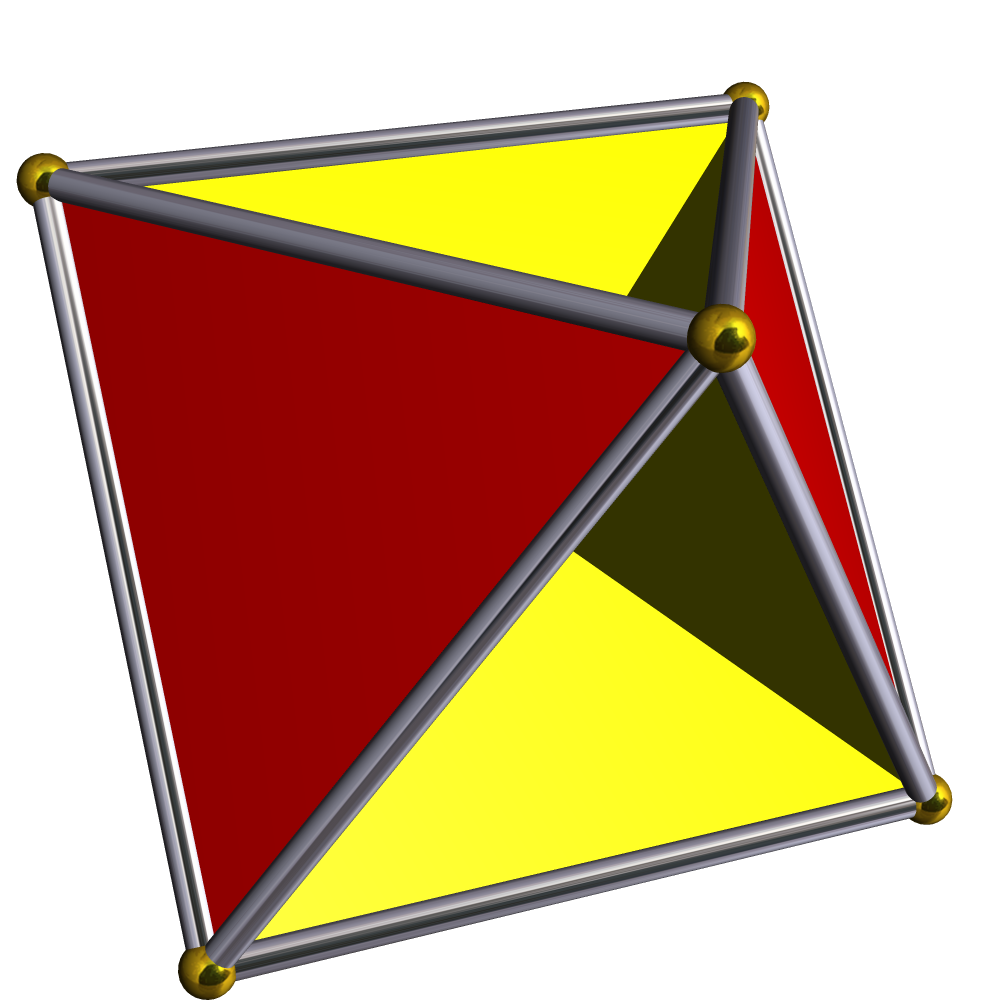
\includegraphics{Figures/Tetrahemihexahedron.png}
%https://en.wikipedia.org/wiki/Euler_characteristic#/media/File:Tetrahemihexahedron.png
\caption[Tetrahemihexaedro]{Tetrahemihexaedro regular. Algunas de sus caras se
intersecan entre sí, haciendo que su topología sea diferente a la de la bola
cerrada. Imagen: \cite{Tetra}.}
\end{marginfigure}

Un espacio topológico $X \subset \mb{R}^n$ 2AN y Hausdorff es una superficie
si, dado $p \in X$, existe un entorno abierto $U \subset X$ de $p$ homeomorfo
a una bola de $\mb{R}^2$. Desde un punto de vista geométrico, podemos decir
que los puntos de $X$ perciben el mundo en dos dimensiones, al igual que los
personajes de la novela \emph{Planilandia}. Algunas superficies pueden ser
representadas utilizando poliedros regulares, que podemos clasificar en
función de su característica de Euler. Cuando una superficie sea homeomorfa a
algún poliedro regular, diremos que es poliédrica.

A partir de un espacio topológico, podemos generar una familia de grupos
abelianos llamados \emph{grupos de homología}. Los grupos de homología nos
permiten utilizar técnicas de álgebra conmutativa para conocer algunas de las
propiedades topológicas de un espacio, permitiendo probar resultados que están
fuera del alcance de la topología conjuntista. En particular, veremos una
demostración del teorema del punto fijo de Brouwer, que establece la
existencia de puntos fijos para cualquier aplicación continua entre conjuntos
convexos.

Este texto está fuertemente basado en \cite{Vick94}, un texto dirigido a
estudiantes de máster y doctorado (conocido en Estados Unidos como el
\emph{graduate level}), por lo que las explicaciones son más breves y muchos
detalles se asumen triviales. Mi objetivo es adaptar estos textos, de
forma que sean lo más asequible posible a estudiantes de 3º y 4º de carrera.

Dado que la información en \cite{Vick94} está muy concentrada, se han tomado
los dos primeros capítulos y convertido en partes. Se recomienda al lector
tratar de entender y computar ejemplos antes de pasar a la parte siguiente.

La primera parte de este texto corresponde al capítulo 1, \emph{Singular
Homology Theory}, donde se introducen los grupos de homología singular y las
sucesiones de Mayer-Vietoris. Las sucesiones de Mayer-Vietoris son la técnica
básica para calcular los grupos de homología de un espacio topológico, y
son válidas para cualquier espacio.

La segunda parte corresponde al capítulo 2, \emph{Attaching Spaces with Maps},
donde se introducen los espacios CW-complejos y los grupos de homología
celular. La homología celular es una forma más directa de computar los grupos
de homología, pero requiere que nuestro espacio admita una estructura especial,
la \emph{estratificación por CW-complejos}.

Finalmente, los apéndices presentan información adicional que no es necesaria
para poder seguir el texto, pero he considerado interesante y digma de
discusión.

El objetivo de este texto es introducir al lector en la teoría de homología
singular, y está dirigido principalmente a estudiantes de la \emph{Universitat
de València}. Como consecuencia, el lector se asume familiarizado con el
contenido cubierto por las asignaturas de Estructuras algebraicas y Topología
de segundo curso.


\pagelayout{wide} % No margins
\addpart{Class Options, Commands and Environments}
\pagelayout{margin} % Restore margins

\setchapterpreamble[u]{\margintoc}
\chapter{Class Options}
\labch{options}

In this chapter I will describe the most common options used, both the 
ones inherited from \Class{scrbook} and the \Class{kao}-specific ones. 
Options passed to the class modifies its default behaviour; beware 
though that some options may lead to unexpected results\ldots

\section{\Class{KOMA} Options}

The \Class{kaobook} class is based on \Class{scrbook}, therefore it 
understands all of the options you would normally pass to that class. If 
you have a lot of patience, you can read the \KOMAScript\xspace 
guide.\sidenote{The guide can be downloaded from 
\url{https://ctan.org/pkg/koma-script?lang=en}.} Actually, the reading 
of such guide is suggested as it is very instructive.

Every \KOMAScript\xspace option you pass to the class when you load it 
is automatically activated. In addition, in \Class{kaobook} some options 
have modified default values. For instance, the font size is 9.5pt and 
the paragraphs are separated by space,\sidenote[][-7mm]{To be precise, 
they are separated by half a line worth of space: the \Option{parskip} 
value is \enquote{half}.} not marked by indentation.

\section{\Class{kao} Options}

In the future I plan to add more options to set the paragraph formatting 
(justified or ragged) and the position of the margins (inner or outer in 
twoside mode, left or right in oneside mode).\sidenote{As of now, 
paragraphs are justified, formatted with \Command{singlespacing} (from 
the \Package{setspace} package) and \Command{frenchspacing}.}

I take this opportunity to renew the call for help: everyone is 
encouraged to add features or reimplement existing ones, and to send me 
the results. You can find the GitHub repository at 
\url{https://github.com/fmarotta/kaobook}.

\begin{kaobox}[frametitle=To Do]
Implement the \Option{justified} and \Option{margin} options. To be 
consistent with the \KOMAScript\xspace style, they should accept a 
simple switch as a parameter, where the simple switch should be 
\Option{true} or \Option{false}, or one of the other standard values for 
simple switches supported by \KOMAScript. See the \KOMAScript\xspace 
documentation for further information.
\end{kaobox}

The above box is an example of a \Environment{kaobox}, which will be 
discussed more thoroughly in \frefch{mathematics}. Throughout the book I 
shall use these boxes to remarks what still needs to be done.

\section{Other Things Worth Knowing}

A bunch of packages are already loaded in the class because they are 
needed for the implementation. These include:

\begin{itemize}
	\item etoolbox
	\item calc
	\item xifthen
	\item xkeyval
	\item xparse
	\item xstring
\end{itemize}

Many more packages are loaded, but they will be discussed in due time. 
Here, we will mention only one more set of packages, needed to change 
the paragraph formatting (recall that in the future there will be 
options to change this). In particular, the packages we load are:

\begin{itemize}
	\item ragged2e
	\item setspace
	\item hyphenat
	\item microtype
	\item needspace
	\item xspace
	\item xcolor (with options \Option{usenames,dvipsnames})
\end{itemize}

Some of the above packages do not concern paragraph formatting, but we 
nevertheless grouped them with the others. By default, the main text is 
justified and formatted with singlespacing and frenchspacing; the margin 
text is the same, except that the font is a bit smaller.

As a last warning, please be aware that the \Package{cleveref} package 
is not compatible with \Class{kaobook}. You should use the commands 
discussed in \refsec{hyprefs} instead.

\section{Document Structure}

We provide optional arguments to the \Command{title} and 
\Command{author} commands so that you can insert short, plain text 
versions of this fields, which can be used, typically in the half-title 
or somewhere else in the front matter, through the commands 
\Command{@plaintitle} and \Command{@plainauthor}, respectively. The PDF 
properties \Option{pdftitle} and \Option{pdfauthor} are automatically 
set by hyperref to the plain values if present, otherwise to the normal 
values.\sidenote[][*-1]{We think that this is an important point so 
we remark it here. If you compile the document with pdflatex, the PDF 
metadata will be altered so that they match the plain title and author 
you have specified; if you did not specify them, the metadata will be 
set to the normal title and author.}

There are defined two page layouts, \Option{margin} and \Option{wide}, 
and two page styles, \Option{plain} and \Option{fancy}. The layout 
basically concern the width of the margins, while the style refers to 
headers and footer; these issues will be 
discussed in \frefch{layout}.\sidenote[][6mm]{For now, suffice it to say that pages with 
the \Option{margin} layout have wide margins, while with the 
\Option{wide} layout the margins are absent. In \Option{plain} pages the 
headers and footer are suppressed, while in \Option{fancy} pages there 
is a header.} 

The commands \Command{frontmatter}, \Command{mainmatter}, and 
\Command{backmatter} have been redefined in order to automatically 
change page layout and style for these sections of the book. The front 
matter uses the \Option{margin} layout and the \Option{plain} page 
style. In the mainmatter the margins are wide and the headings are 
fancy. In the appendix the style and the layout do not change; however 
we use \Command{bookmarksetup\{startatroot\}} so that the bookmarks of 
the chapters are on the root level (without this, they would be under 
the preceding part). In the backmatter the margins shrink again and we 
also reset the bookmarks root.

\setchapterpreamble[u]{\margintoc}
\chapter{Margin Stuff}

Sidenotes are a distinctive feature of all 1.5-column-layout books. 
Indeed, having wide margins means that some material can be displayed 
there. We use margins for all kind of stuff: sidenotes, marginnotes, 
small tables of contents, citations, and, why not?, special boxes and 
environments.

\section{Sidenotes}

Sidenotes are like footnotes, except that they go in the margin, where 
they are more readable. To insert a sidenote, just use the command 
\Command{sidenote\{Text of the note\}}. You can specify a 
mark\sidenote[O]{This sidenote has a special mark, a big O!} with \\ 
\Command{sidenote[mark]\{Text\}}, but you can also specify an offset, 
which moves the sidenote upwards or downwards, so that the full syntax is:

\begin{lstlisting}[style=kaolstplain]
\sidenote[mark][offset]{Text}
\end{lstlisting}

If you use an offset, you always have to add the brackets for the mark, 
but they can be empty.\sidenote{If you want to know more about the usage 
of the \Command{sidenote} command, read the documentation of the 
\Package{sidenotes} package.}

In \Class{kaobook} we copied a feature from the \Package{snotez} 
package: the possibility to specify a multiple of \Command{baselineskip} 
as an offset. For example, if you want to enter a sidenote with the 
normal mark and move it upwards one line, type:

\begin{lstlisting}[style=kaolstplain]
\sidenote[][*-1]{Text of the sidenote.}
\end{lstlisting}

As we said, sidenotes are handled through the \Package{sidenotes} 
package, which in turn relies on the \Package{marginnote} package.

\section{Marginnotes}

This command is very similar to the previous one. You can create a 
marginnote with \Command{marginnote[offset]\{Text\}}, where the offset 
argument can be left out, or it can be a multiple of 
\Command{baselineskip},\marginnote[-1cm]{While the command for margin 
notes comes from the \Package{marginnote} package, it has been redefined 
in order to change the position of the optional offset argument, which 
now precedes the text of the note, whereas in the original version it 
was at the end. We have also added the possibility to use a multiple of 
\Command{baselineskip} as offset. These things were made only to make 
everything more consistent, so that you have to remember less things!} 
\eg

\begin{lstlisting}[style=kaolstplain]
\marginnote[-12pt]{Text} or \marginnote[*-3]{Text}
\end{lstlisting}

\begin{kaobox}[frametitle=To Do]
A small thing that needs to be done is to renew the \Command{sidenote} 
command so that it takes only one optional argument, the offset. The 
special mark argument can go somewhere else. In other words, we want the 
syntax of \Command{sidenote} to resemble that of \Command{marginnote}.
\end{kaobox}

We load the packages \Package{marginnote}, \Package{marginfix} and 
\Package{placeins}. Since \Package{sidenotes} uses \Package{marginnote}, 
what we said for marginnotes is also valid for sidenotes. Side- and 
margin- notes are shifted slightly upwards 
(\Command{renewcommand\{\textbackslash marginnotevadjust\}\{3pt\}}) in 
order to allineate them to the bottom of the line of text where the note 
is issued.

\section{Footnotes}

Even though they are not displayed in the margin, we will discuss about 
footnotes here, since sidenotes are mainly intended to be a replacement 
of them. Footnotes force the reader to constantly move from one area of 
the page to the other. Arguably, marginnotes solve this issue, so you 
should not use footnotes. Nevertheless, for completeness, we have left 
the standard command \Command{footnote}, just in case you want to put a 
footnote once in a while.\footnote{And this is how they look like. 
Notice that in the PDF file there is a back reference to the text; 
pretty cool, uh?}

\section{Margintoc}

Since we are talking about margins, we introduce here the 
\Command{margintoc} command, which allows one to put small table of 
contents in the margin. Like other commands we have discussed, 
\Command{margintoc} accepts a parameter for the vertical offset, like 
so: \Command{margintoc[offset]}.

The command can be used in any point of the document, but we think it 
makes sense to use it just at the beginning of chapters or parts. In 
this document I make use of a \KOMAScript\xspace feature and put it in 
the chapter preamble, with the following code:

\marginnote{The font used in the margintoc is the same as the one for 
	the chapter entries in the main table of contents at the beginning 
	of the document.}

\begin{lstlisting}[style=kaolstplain]
\setchapterpreamble[u]{\margintoc}
\chapter{Chapter title}
\end{lstlisting}

\section{Marginlisting}

On some occasions it may happen that you have a very short piece of code 
that doesn't look good in the body of the text because it breaks the 
flow of narration: for that occasions, you can use a 
\Environment{marginlisting}. The support for this feature is still 
limited, especially for the captions, but you can try the following 
code:

\begin{marginlisting}[-1.35cm]
	\caption{An example of a margin listing.}
	\vspace{0.6cm}
	\begin{lstlisting}[language=Python,style=kaolstplain]
print("Hello World!")
	\end{lstlisting}
\end{marginlisting}

\begin{verbatim}
\begin{marginlisting}[-0.5cm]
	\caption{My caption}
	\vspace{0.2cm}
	\begin{lstlisting}[language=Python,style=kaolstplain]
	... code ...
	\end{lstlisting}
\end{marginlisting}
\end{verbatim}

Unfortunately, the space between the caption and the listing must be 
adjusted manually; if you find a better way, please let me know.

Not only textual stuff can be displayed in the margin, but also figures. 
Those will be the focus of the next chapter.

\setchapterimage[6.5cm]{seaside}
\setchapterpreamble[u]{\margintoc}
\chapter[Figures and Tables]{Figures and Tables\footnotemark[0]}

\footnotetext{The credits for the image above the chapter title go to:
	Bushra Feroz --- Own work, CC~BY-SA~4.0, 
	\url{https://commons.wikimedia.org/w/index.php?curid=68724647}}

\section{Normal Figures and Tables}

Figures and tables can be inserted just like in any standard 
\LaTeX\xspace document. The \Package{graphicx} package is already loaded 
and configured in such a way that the figure width is equal to the 
textwidth and the height is adjusted in order to maintain the original 
aspect ratio. As you may have imagined, the captions will be 
positioned\ldots well, in the margins. This is achieved with the help of 
the \Package{floatrow} package.

Here is a picture of Mona Lisa (\reffig{normalmonalisa}), as an example. 
The captions are formatted as the margin- and the side-notes; If you 
want to change something about captions you can use the command 
\Command{captsetup} from the \Package{caption} package. Remember that if 
you want to reference a figure, the label must come \emph{after} the 
caption!

\begin{figure}[hb]
	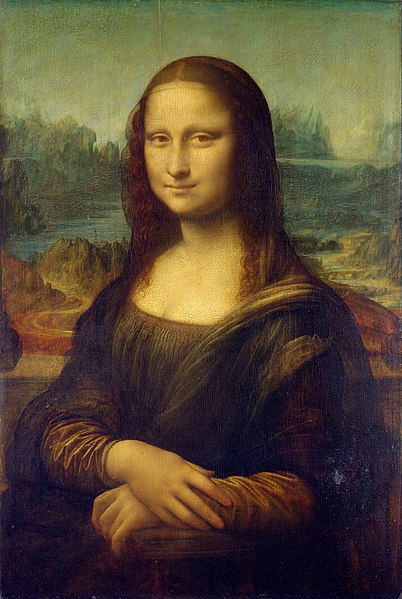
\includegraphics[width=0.45\textwidth]{monalisa}
	\caption[Mona Lisa, again]{It's Mona Lisa again. \blindtext}
	\labfig{normalmonalisa}
\end{figure}

While the format of the caption is managed by \Package{caption}, its 
position is handled by the \Package{floatrow} package. Achieving this 
result has been quite hard, but now I am pretty satisfied. In two-side 
mode, the captions are printed in the correct margin.

Tables can be inserted just as easily as figures, as exemplified by the 
following code:

\begin{lstlisting}[caption={Caption of a listing.}]
\begin{table}
\begin{tabular}{ c c c c }
	\toprule
	col1 & col2 & col3 & col 4 \\
	\midrule
	\multirow{3}{4em}{Multiple row} & cell2 & cell3 & cell4\\ &
	cell5 & cell6 & cell7 \\ &
	cell8 & cell9 & cell10 \\
	\multirow{3}{4em}{Multiple row} & cell2 & cell3 & cell4 \\ &
	cell5 & cell6 & cell7 \\ &
	cell8 & cell9 & cell10 \\
	\bottomrule
\end{tabular}
\end{table}
\end{lstlisting}

which results in the useless \vreftab{useless}.

\begin{table}[h]
\caption[A useless table]{A useless table.}
\labtab{useless}
\begin{tabular}{ c c c c }
	\toprule
	col1 & col2 & col3 & col 4 \\
	\midrule
	\multirow{3}{4em}{Multiple row} & cell2 & cell3 & cell4\\ &
	cell5 & cell6 & cell7 \\ &
	cell8 & cell9 & cell10 \\
	\multirow{3}{4em}{Multiple row} & cell2 & cell3 & cell4 \\ &
	cell5 & cell6 & cell7 \\ &
	cell8 & cell9 & cell10 \\
	\bottomrule
\end{tabular}
\end{table}

I don't have much else to say, so I will just insert some blind text. 
\blindtext

\section{Margin Figures and Tables}

Marginfigures can be inserted with the environment 
\Environment{marginfigure}. In this case, the whole picture is confined 
to the margin and the caption is below it. \reffig{marginmonalisa} is 
obtained with something like this:

\begin{lstlisting}[caption={Another caption.}]
\begin{marginfigure}
	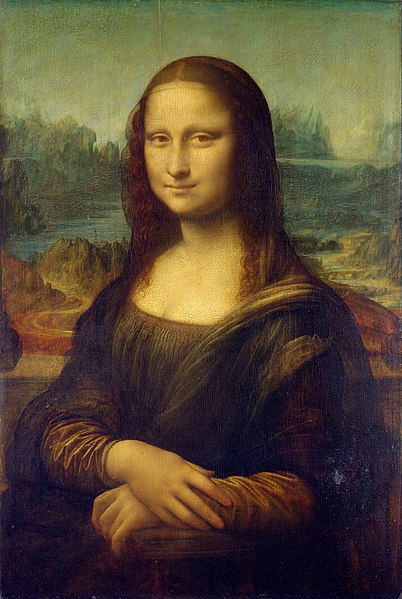
\includegraphics{monalisa}
	\caption[The Mona Lisa]{The Mona Lisa.}
	\labfig{marginmonalisa}
\end{marginfigure}
\end{lstlisting}

There is also the \Environment{margintable} environment, of which 
\reftab{anotheruseless} is an example. Notice how you can place the 
caption above the table by just placing the \Command{caption} command 
before beginning the \Environment{tabular} environment. Usually, figure 
captions are below, while table captions are above. This rule is also 
respected for normal figures and tables: the captions are always on the 
side, but for figure they are aligned to the bottom, while for tables to 
the top.

\begin{margintable}
\caption[Another useless table]{Another useless table.}
\labtab{anotheruseless}
\raggedright
\begin{tabular}{ c c c c }
	\hline
	col1 & col2 & col3 \\
	\hline
	\multirow{3}{4em}{Multiple row} & cell2 & cell3 \\ & cell5 & cell6 
	\\ & cell8 & cell9 \\ \hline
\end{tabular}
\end{margintable}

Marginfigures and tables can be positioned with an optional offset 
command, like so:

\begin{lstlisting}
\begin{marginfigure}[offset]
	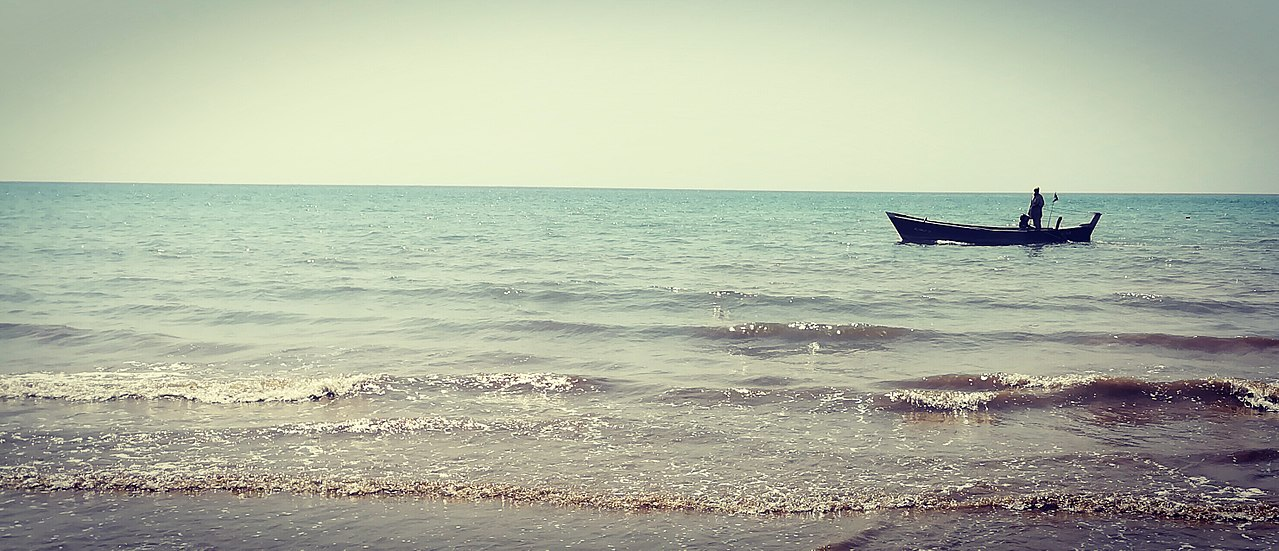
\includegraphics{seaside}
\end{marginfigure}
\end{lstlisting}

Offset ca be either a measure or a multiple of \Command{baselineskip}, 
much like with \Command{sidenote}, \Command{marginnote} and 
\Command{margintoc}.\todo{Improve this part.} If you are wondering how I 
inserted this orange bubble, have a look at the \Package{todo} package.

\section{Wide Figures and Tables}

\begin{figure*}[h!]
	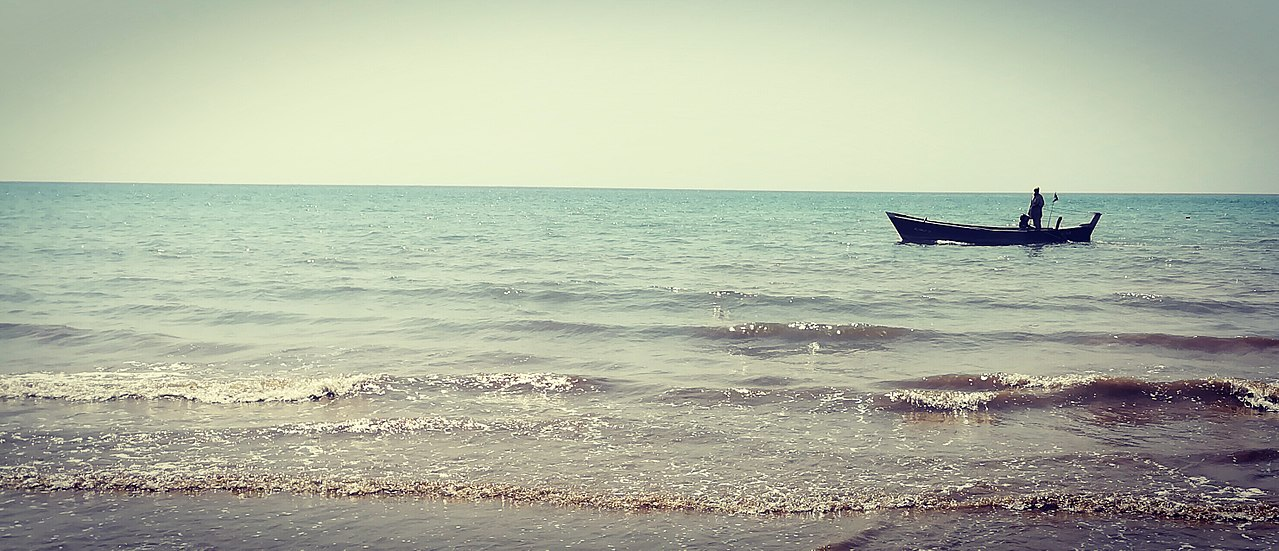
\includegraphics{seaside}
	\caption[A wide seaside]{A wide seaside, and a wide caption.
		Credits: By Bushra Feroz --- Own work, CC BY-SA 4.0, 
		\url{https://commons.wikimedia.org/w/index.php?curid=68724647}}
\end{figure*}

With the environments \Environment{figure*} and \Environment{table*} you 
can insert figures which span the whole page width. The caption will be 
positioned below or above, according to taste.

You may have noticed the full width image at the very beginning of this 
chapter: that, however, is set up in an entirely different way, which 
you'll read about in \vrefch{layout}. Now it is time to tackle 
hyperreferences.

\setchapterstyle{kao}
%\setchapterpreamble[u]{\margintoc}
\chapter{References}
\labch{references}

\section{Citations}

\index{citations}
To cite someone \sidecite{Visscher2008,James2013} is very simple: just 
use the \Command{sidecite}\index{\Command{sidecite}} command. It does 
not have an offset argument yet, but it probably will in the future. 
This command supports multiple entries, as you can see, and by default 
it prints the reference on the margin as well as adding it to the 
bibliography at the end of the document. Note that the citations have 
nothing to do with the text,\sidecite{James2013} but they are completely 
random as they only serve the purpose to illustrate the feature.

For this setup I wrote a separate package, \Package{kaobiblio}, which 
you can find in the \Package{styles} directory and include in your main 
tex file. This package accepts all the options that you can pass to 
\Package{biblatex}, and actually it passes them to \Package{biblatex} 
under the hood. Moreover, it also defines some commands, like 
\Command{sidecite}, and environments that can be used within a 
\Class{kao} book.\sidenote{For this reason you should always use 
\Package{kaobiblio} instead of \Package{biblatex}, but the syntax and 
the options are exactly the same.}

As you have seen, the \Command{sidecite} command will print a citation 
in the margin. However, this command would be useless without a way to 
customise the format of the citation, so the \Class{kaobook} provides 
also the \Command{formatmargincitation} command. By \enquote{renewing} 
that command, you can choose which items will be printed in the margins. 
The best way to understand how it works is to see the actual definition 
of this command.

\begin{lstlisting}[style=kaolstplain,linewidth=1.5\textwidth]
\newcommand{\formatmargincitation}[1]{
	\parencite{#1}: \citeauthor*{#1} (\citeyear{#1}), \citetitle{#1}\\
}
\end{lstlisting}

Thus, the \Command{formatmargincitation} accepts one parameter, which is 
the citation key, and prints the parencite followed by a colon, then the 
author, then the year (in brackets), and finally the 
title.\sidecite{Battle2014} Now, suppose that you wish the margin 
citation to display the year and the author, followed by the title, and 
finally a fixed arbitrary string; you would add to your document:

\begin{lstlisting}[style=kaolstplain,linewidth=1.5\textwidth]
\renewcommand{\formatmargincitation}[1]{
	\citeyear{#1}, \citeauthor*{#1}: \citetitle{#1}; very interesting!\\
}
\end{lstlisting}

\renewcommand{\formatmargincitation}[1]{
	\citeyear{#1}, \citeauthor*{#1}: \citetitle{#1}; very interesting!\\
}

The above code results in citations that look like the 
following.\sidecite{Zou2005} Of course, changing the format is most 
useful when you also change the default bibliography style. For 
instance, if you want to use the \enquote{philosophy-modern} style for 
your bibliography, you might have something like this in the preamble:

\begin{lstlisting}[style=kaolstplain,linewidth=1.5\textwidth]
\usepackage[style=philosophy-modern]{styles/kaobiblio}
\renewcommand{\formatmargincitation}[1]{
	\sdcite{#1}\\
}
\addbibresource{main.bib}
\end{lstlisting}

\renewcommand{\formatmargincitation}[1]{
	\parencite{#1}: \citeauthor*{#1} (\citeyear{#1}), \citetitle{#1}\\
}

The commands like \Command{citeyear}, \Command{parencite} and 
\Command{sdcite} are just examples. A full reference of the available 
commands can be found in this 
\href{http://tug.ctan.org/info/biblatex-cheatsheet/biblatex-cheatsheet.pdf}{cheatsheet}, 
under the \enquote{Citations} section.

Finally, to compile a document containing citations, you need to use an 
external tool, which for this class is biber. You need to run the 
following (assuming that your tex file is called main.tex):

\begin{lstlisting}[style=kaolstplain]
$ pdflatex main
$ biber main
$ pdflatex main
\end{lstlisting}

\section{Glossaries and Indices}

\index{glossary}
The \Class{kaobook} class loads the packages \Package{glossaries} and 
\Package{imakeidx}, with which you can add glossaries and indices to 
your book. For instance, I previously defined some glossary entries and 
now I am going to use them, like this: \gls{computer}. 
\Package{glossaries} also allows you to use acronyms, like the 
following: this is the full version, \acrfull{fpsLabel}, and this is the 
short one \acrshort{fpsLabel}. These entries will appear in the glossary 
in the backmatter.

Unless you use \href{https://www.overleaf.com}{Overleaf} or some other 
fancy IDE for \LaTeX, you need to run an external command from your 
terminal in order to compile a document with a glossary. In particular, 
the commands required are:\sidenote{These are the commands you 
would run in a UNIX system; I have no idea on how it works in Windows.}

\begin{lstlisting}[style=kaolstplain]
$ pdflatex main
$ makeglossaries main
$ pdflatex main
\end{lstlisting}

Note that you need not run \texttt{makeglossaries} every time you 
compile your document, but only when you change the glossary entries.

\index{index}
To create an index, you need to insert the command 
\lstinline|\index{subject}| whenever you are talking about 
\enquote{subject} in the text. For instance, at the start of this 
paragraph I would write \lstinline|index{index}|, and an entry would be 
added to the Index in the backmatter. Check it out!

\marginnote[2mm]{In theory, you would need to run an external command 
for the index as well, but luckily the package we suggested, 
	\Package{imakeidx}, can compile the index automatically.}

\index{nomenclature}
A nomenclature is just a special kind of index; you can find one at the end of
this book. To insert a nomenclature, we use the package \Package{nomencl} and
add the terms with the command \Command{nomenclature}. We put then a
\Command{printnomenclature} where we want it to appear.

Also with this package we need to run an external command to compile the 
document, otherwise the nomenclature will not appear:

\begin{lstlisting}[style=kaolstplain]
$ pdflatex main
$ makeindex main.nlo -s nomencl.ist -o main.nls
$ pdflatex main
\end{lstlisting}

These packages are all loaded in 
\href{style/packages.sty}{packages.sty}, one of the files that come with 
this class. However, the configuration of the elements is best done in 
the main.tex file, since each book will have different entries and 
styles.

Note that the \Package{nomencl} package caused problems when the 
document was compiled, so, to make a long story short, I had to prevent 
\Package{scrhack} to load the hack-file for \Package{nomencl}. When 
compiling the document on Overleaf, however, this problem seem to 
vanish.

\marginnote[-19mm]{This brief section was by no means a complete 
reference on the subject, therefore you should consult the documentation 
of the above package to gain a full understanding of how they work.}

\section{Hyperreferences}
\labsec{hyprefs}

\index{hyperreferences}
In this class we provide a handy sub-package to help you referencing the 
same elements always in the same way, for consistency across the book. 
First, you can label each element with a specific command. For instance, 
should you want to label a chapter, you would put 
\lstinline|\labch{chapter-title}| right after the \Command{chapter} 
directive. This is just a convienence, because \Command{labch} is 
actually just an alias to \lstinline|\label{ch:chapter-title}|, so it 
spares you the writing of \enquote{ch}. We defined similar commands for 
many typically labeled elements, including:

\begin{multicols}{2}
\setlength{\columnseprule}{0pt}
\begin{itemize}
	\item Page: \Command{labpage}
	\item Part: \Command{labpart}
	\item Chapter: \Command{labch}
	\item Section: \Command{labsec}
	\item Figure: \Command{labfig}
	\item Table: \Command{labtab}
	\item Definition: \Command{labdef}
	\item Theorem: \Command{labthm}
	\item Proposition: \Command{labprop}
	\item Lemma: \Command{lablemma}
	\item Remark: \Command{labremark}
	\item Example: \Command{labexample}
	\item Exercise: \Command{labexercise}
\end{itemize}
\end{multicols}

Of course, we have similar commands for referencing those elements. 
However, since the style of the reference should depend on the context, 
we provide different commands to reference the same thing. For instance, 
in some occasions you may want to reference the chapter by name, but 
other times you want to reference it only by number. In general, there 
are four reference style, which we call plain, vario, name, and full. 

The plain style references only by number. It is accessed, for chapters, 
with \lstinline|\refch{chapter-title}| (for other elements, the syntax 
is analogous). Such a reference results in: \refch{references}.

The vario and name styles rest upon the \Package{varioref} package. 
Their syntax is \lstinline|\vrefch{chapter-title}| and 
\lstinline|\nrefch{chapter-title}|, and they result in: 
\vrefch{references}, for the vario style, and: \nrefch{references}, for 
the name style. As you can see, the page is referenced in 
\Package{varioref} style.

The full style references everything. You can use it with 
\lstinline|\frefch{chapter-title}| and it looks like this: 
\frefch{references}.

Of course, all the other elements have similar commands (\eg for parts 
you would use \lstinline|\vrefpart{part-title}| or something like that). 
However, not all elements implement all the four styles. The commands 
provided should be enough, but if you want to see what is available or 
to add the missing ones, have a look at the 
\href{styles/kaorefs.sty}{attached package}.


\pagelayout{wide} % No margins
\addpart{Design and Additional Features}
\pagelayout{margin} % Restore margins

\setchapterimage[6cm]{seaside}
\setchapterpreamble[u]{\margintoc}
\chapter{Page Design}
\labch{layout}

\section{Headings}

So far, in this document I used two different styles for the chapter 
headings: one has the chapter name, a rule and, in the margin, the 
chapter number; the other has an image at the top of the page, and the 
chapter title is printed in a box (like for this chapter). There is one 
additional style, which I used only in the appendix 
(\vrefpage{appendix}); there, the chapter title is enclosed in two 
horizontal rules, and the chapter number (or letter, in the case of the 
appendix) is above it.\sidenote{To be honest, I do not think that mixing 
heading styles like this is a wise choice, but in this document I did it 
only to show you how they look.}

Every book is unique, so it makes sense to have different styles from 
which to choose. Actually, it would be awesome if whenever a 
\Class{kao}-user designs a new heading style, he or she added it to the 
three styles already present, so that it will be available for new users 
and new books.

The choice of the style is made simple by the \Command{setchapterstyle} 
command. It accepts one option, the name of the style, which can be: 
\enquote{plain}, \enquote{kao}, or \enquote{lines}.\sidenote{Plain is 
the default \LaTeX\xspace title style; the other ones are self 
explanatory.} If instead you want the image style, you have to use the 
command \Command{setchapterimage}, which accepts the path to the image 
as argument; you can also provide an optional parameter in square 
brackets to specify the height of the image.

Let us make some examples. In this book, I begin a normal chapter with 
the lines:

\begin{lstlisting}
\setchapterstyle{kao}
\setchapterpreamble[u]{\margintoc}
\chapter{Title of the Chapter}
\labch{title}
\end{lstlisting}

In Line 1 I choose the style for the title to be \enquote{kao}. Then, I 
specify that I want the margin toc. The rest is ordinary administration 
in \LaTeX, except that I use my own \Command{labch} to label the 
chapter. Actually, the \Command{setchapterpreamble} is a standard 
\KOMAScript\xspace one, so I invide you to read about it in the KOMA 
documentation. Once the chapter style is set, it holds until you change 
it.\sidenote{The \Command{margintoc} has to be specified at every 
chapter. Perhaps in the future this may change; it all depends on how 
this feature will be welcomed by the users, so keep in touch with me if 
you have preferences!} Whenever I want to start a chapter with an image, 
I simply write:

\begin{lstlisting}
\setchapterimage[7cm]{path/to/image.png} % Optionally specify the height
\setchapterpreamble[u]{\margintoc}
\chapter{Catchy Title} % No need to set a chapter style
\labch{catchy}
\end{lstlisting}

If you prefer, you can also specify the style at the beginning of the 
main document, and that style will hold until you change it again.

\section{Headers \& Footers}

Headers and footers in \KOMAScript\xspace are handled by the 
\Package{scrlayer-scrpage} package. There are two basic style: 
\enquote{scrheadings} and \enquote{plain.scrheadings}. The former is 
used for normal pages, whereas the latter is used in title pages (those 
where a new chapter starts, for instance) and, at least in this book, in 
the front matter. At any rate, the style can be changed with the 
\Command{pagestyle} command, \eg 
\lstinline|\pagestyle{plain.scrheadings}|.

In both stles, the footer is completely empty. In plain.scrheadings, 
also the header is absent (otherwise it wouldn't be so plain\ldots), but 
in the normal style the design is reminescent of the \enquote{kao} style 
for chapter titles.

\begin{kaobox}[frametitle=To Do]
The \Option{twoside} class option is still unstable and may lead to 
unexpected behaviours. As always, any help will be greatly appreciated.
\end{kaobox}

\section{Table of Contents}

Another important part of a book is the table of contents. By default, 
in \Class{kaobook} there is an entry for everything: list of figures, 
list of tables, bibliographies, and even the table of contents itself. 
Not everybody might like this, so we will provide a description of the 
changes you need to do in order to enable or disable each of these 
entries. In the following \reftab{tocentries}, each item corresponds to 
a possible entry in the \acrshort{tocLabel}, and its description is the 
command you need to provide to have such entry. These commands are 
specified in the attached \href{style/style.sty}{style 
package},\sidenote{In the same file, you can also choose the titles of 
these entries.} so if you don't want the entries, just comment the 
corresponding lines.

Of course, some packages, like those for glossaries and indices, will 
try to add their own entries.\marginnote{In a later section, we will see 
how you can define your own floating environment, and endow it with an 
entry in the \acrshort{tocLabel}.} In such cases, you have to follow the 
instructions specific to that package. Here, since we have talked about 
glossaries and notations in \refch{references}, we will biefly see how 
to configure them.

\begin{table}
\footnotesize
\caption{Commands to add a particular entry to the table of contents.}
\labtab{tocentries}
\begin{tabular}{ l l }
	\toprule
	Entry & Command to Activate \\
	\midrule
	Table of Contents & \lstinline|\setuptoc{toc}{totoc}| \\
	List of Figs and Tabs & \lstinline|\PassOptionsToClass{toc=listof}{\@baseclass}| \\
	Bibliography & \lstinline|\PassOptionsToClass{toc=bibliography}{\@baseclass}| \\
	\bottomrule
\end{tabular}
\end{table}

For the \Package{glossaries} package, use the \enquote{toc} option when 
you load it: \lstinline|\usepackage[toc]{glossaries}|. For 
\Package{nomencl}, pass the \enquote{intoc} option at the moment of 
loading the package. Both \Package{glossaries} and \Package{nomencl} are 
loaded in the attached \href{style/packages.sty}{\enquote{packages} 
package}.

Additional configuration of the table of contents can be performed 
through the packages \Package{etoc}, which is loaded because it is 
needed for the margintocs, or the more traditional \Package{tocbase}. 
Read the respective documentations if you want to be able to change the 
default \acrshort{tocLabel} style.\sidenote[][*-1]{(And please, send me 
a copy of what you have done, I'm so curious!)}

\section{Page Layout}

Besides the page style, you can also change the width of the content of 
a page. This is particularly useful for pages dedicated to part titles, 
where having the 1.5-column layout might be a little awkward, or for 
pages where you only put figures, where it is important to exploit all 
the available space.

In practice, there are two layouts: \enquote{wide} and \enquote{margin}. 
The former suppresses the margins and allocates the full page for 
contents, while the latter is the layout used in most of the pages of 
this book, including this one. The wide layout is also used 
automatically in the front and back matters.

To change page layout, use the \Command{pagelayout} command. For 
example, when I start a new part, I write:

\begin{lstlisting}
\pagelayout{wide}
\addpart{Title of the New Part}
\pagelayout{margin}
\end{lstlisting}

\section{Numbers \& Counters}

In this short section we shall see how dispositions, sidenotes and 
figures are numbered in the \Class{kaobook} class.

By default, dispositions are numbered up to the section. This is 
achieved by setting: \lstinline|\setcounter{secnumdepth}{1}|.

The sidenotes counter is the same across all the document, but if you 
want it to reset at each chapter, just uncomment the line

\begin{lstlisting}[style=kaolstplain]
\counterwithin*{sidenote}{chapter}
\end{lstlisting}

in the \Package{styles/style.sty} package provided by this class.

Figure and Table numbering is also per-chapter; to change that, use 
something like:

\begin{lstlisting}[style=kaolstplain]
\renewcommand{\thefigure}{\arabic{section}.\arabic{figure}}
\end{lstlisting}

\section{White Space}

One of the things that I find most hard in \LaTeX\xspace is to finely 
tune the white space around objects. There are not fixed rules, each 
object needs its own adjustment. Here we shall see how some spaces are 
defined at the moment in this class.\marginnote{Attention! This section 
may be incomplete.}

\textbf{Space around figures and tables}

\begin{lstlisting}[style=kaolstplain]
\renewcommand\FBaskip{.4\topskip}
\renewcommand\FBbskip{\FBaskip}
\end{lstlisting}

\textbf{Space around captions}

\begin{lstlisting}[style=kaolstplain]
\captionsetup{
	aboveskip=6pt,
	belowskip=6pt
}
\end{lstlisting}

\textbf{Space around displays (\eg equations)}

\begin{lstlisting}[style=kaolstplain]
\setlength\abovedisplayskip{6pt plus 2pt minus 4pt}
\setlength\belowdisplayskip{6pt plus 2pt minus 4pt}
\abovedisplayskip 10\p@ \@plus2\p@ \@minus5\p@
\abovedisplayshortskip \z@ \@plus3\p@
\belowdisplayskip \abovedisplayskip
\belowdisplayshortskip 6\p@ \@plus3\p@ \@minus3\p@
\end{lstlisting}

\setchapterstyle{kao}
\setchapterpreamble[u]{\margintoc}
\chapter{Mathematics and Boxes}
\labch{mathematics}

\section{Theorems}

Despite most people complain at the sight of a book full of equations, 
mathematics is an important part of many books. Here, we shall 
illustrate some of the possibilities. We believe that theorems, 
definitions, remarks and examples should be emphasised with a shaded 
background; however, the colour should not be to heavy on the eyes, so 
we have chosen a sort of light yellow.\sidenote{The boxes are all of the 
same colour here, because we did not want our document to look like 
\href{https://en.wikipedia.org/wiki/Harlequin}{Harlequin}.}

\begin{definition}
\labdef{openset}
Let $(X, d)$ be a metric space. A subset $U \subset X$ is an open set 
if, for any $x \in U$ there exists $r > 0$ such that $B(x, r) \subset 
U$. We call the topology associated to d the set $\tau\textsubscript{d}$ 
of all the open subsets of $(X, d).$
\end{definition}

\refdef{openset} is very important. I am not joking, but I have inserted 
this phrase only to show how to reference definitions. The following 
statement is repeated over and over in different environments.

\begin{theorem}
A finite intersection of open sets of (X, d) is an open set of (X, d), 
i.e $\tau\textsubscript{d}$ is closed under finite intersections. Any 
union of open sets of (X, d) is an open set of (X, d).
\end{theorem}

\begin{proposition}
A finite intersection of open sets of (X, d) is an open set of (X, d), 
i.e $\tau\textsubscript{d}$ is closed under finite intersections. Any 
union of open sets of (X, d) is an open set of (X, d).\marginnote{You can even insert footnotes inside the theorem 
	environments; they will be displayed at the bottom of the box.}
\end{proposition}

\begin{lemma}
A finite intersection\footnote{I'm a footnote} of open sets of (X, d) is 
an open set of (X, d), i.e $\tau\textsubscript{d}$ is closed under 
finite intersections. Any union of open sets of (X, d) is an open set of 
(X, d).
\end{lemma}

You can safely ignore the content of the theorems\ldots I assume that if 
you are interested in having theorems in your book, you already know 
something about the classical way to add them. These example should just 
showcase all the things you can do within this class.

\begin{corollary}[Finite Intersection, Countable Union]
A finite intersection of open sets of (X, d) is an open set of (X, d), 
i.e $\tau\textsubscript{d}$ is closed under finite intersections. Any 
union of open sets of (X, d) is an open set of (X, d).
\end{corollary}

\begin{proof}
The proof is left to the reader as a trivial exercise. Hint: \blindtext
\end{proof}

\begin{definition}
Let $(X, d)$ be a metric space. A subset $U \subset X$ is an open set 
if, for any $x \in U$ there exists $r > 0$ such that $B(x, r) \subset 
U$. We call the topology associated to d the set $\tau\textsubscript{d}$ 
of all the open subsets of $(X, d).$\marginnote{
	Here is a random equation, just because we can:
	\begin{equation*}
  x = a_0 + \cfrac{1}{a_1
          + \cfrac{1}{a_2
          + \cfrac{1}{a_3 + \cfrac{1}{a_4} } } }
	\end{equation*}
}
\end{definition}

\begin{example}
Let $(X, d)$ be a metric space. A subset $U \subset X$ is an open set 
if, for any $x \in U$ there exists $r > 0$ such that $B(x, r) \subset 
U$. We call the topology associated to d the set $\tau\textsubscript{d}$ 
of all the open subsets of $(X, d).$
\end{example}

\begin{remark}
Let $(X, d)$ be a metric space. A subset $U \subset X$ is an open set 
if, for any $x \in U$ there exists $r > 0$ such that $B(x, r) \subset 
U$. We call the topology associated to d the set $\tau\textsubscript{d}$ 
of all the open subsets of $(X, d).$
\end{remark}

As you may have noticed, definitions, example and remarks have 
independent counters; theorems, propositions, lemmas and corollaries 
share the same counter.

\begin{remark}
Here is how an integral looks like inline: $\int_{a}^{b} x^2 dx$, and 
here is the same integral displayed in its own paragraph:
\[\int_{a}^{b} x^2 dx\]
\end{remark}

We provide two files for the theorem styles: 
\href{style/plaintheorems.sty}{plaintheorems.sty}, which you should 
include if you do not want coloured boxes around theorems; and 
\href{style/mdftheorems.sty}{mdftheorems.sty}, which is the one used for 
this document.\sidenote{The plain one is not showed, but actually it is 
exactly the same as this one, only without the yellow boxes.} Of course, 
you will have to edit these files according to your taste and the 
general style of the book.

\section[Boxes \& Environments]{Boxes \& Custom Environments
\sidenote[][*1.8]{Notice that in the table of contents and in the 
	header, the name of this section is \enquote{Boxes \& Environments}; 
	we achieved this with the optional argument of the \texttt{section} 
	command.}}

Say you want to insert a special section, an optional content or just 
something you want to emphasise. We think that nothing works better than 
a box in these cases. We used \Package{mdframed} to construct the ones 
shown below. You can create and modify such environments by editing the 
provided file \href{style/environments.sty}{environments.sty}.

\begin{kaobox}[frametitle=Title of the box]
\blindtext
\end{kaobox}

If you set up a counter, you can even create your own numbered 
environment.

\begin{kaocounter}
	\blindtext
\end{kaocounter}

\section{Experiments}

It is possible to wrap marginnotes inside boxes, too. Audacious readers 
are encouraged to try their own experiments and let me know the 
outcomes.

\marginnote[-2.2cm]{
	\begin{kaobox}[frametitle=title of margin note]
		Margin note inside a kaobox.\\
		(Actually, kaobox inside a marginnote!)
	\end{kaobox}
}

I believe that many other special things are possible with the 
\Class{kaobook} class. During its development, I struggled to keep it as 
flexible as possible, so that new features could be added without too 
great an effort. Therefore, I hope that you can find the optimal way to 
express yourselves in writing a book, report or thesis with this class, 
and I am eager to see the outcomes of any experiment that you may try.

%\begin{margintable}
	%\captionsetup{type=table,position=above}
	%\begin{kaobox}
		%\caption{caption}
		%\begin{tabular}{ |c|c|c|c| }
			%\hline
			%col1 & col2 & col3 \\
			%\hline
			%\multirow{3}{4em}{Multiple row} & cell2 & cell3 \\ & cell5 
			%%& cell6 \\ 
			%& cell8 & cell9 \\
			%\hline
		%\end{tabular}
	%\end{kaobox}
%\end{margintable}


\appendix % From here onwards, chapters are numbered with letters, as is the appendix convention

\pagelayout{wide} % No margins
\addpart{Appendix}
\pagelayout{margin} % Restore margins

\setchapterstyle{lines}
\labpage{appendix}
\blinddocument


%----------------------------------------------------------------------------------------

\backmatter % Denotes the end of the main document content
\setchapterstyle{plain} % Output plain chapters from this point onwards

%----------------------------------------------------------------------------------------
%	BIBLIOGRAPHY
%----------------------------------------------------------------------------------------

% The bibliography needs to be compiled with biber using your LaTeX editor, or on the command line with 'biber main' from the template directory

\defbibnote{bibnote}{Here are the references in citation order.\par\bigskip} % Prepend this text to the bibliography
\printbibliography[heading=bibintoc, title=Bibliography, prenote=bibnote] % Add the bibliography heading to the ToC, set the title of the bibliography and output the bibliography note

%----------------------------------------------------------------------------------------
%	NOMENCLATURE
%----------------------------------------------------------------------------------------

% The nomenclature needs to be compiled on the command line with 'makeindex main.nlo -s nomencl.ist -o main.nls' from the template directory

\nomenclature{$c$}{Speed of light in a vacuum inertial frame}
\nomenclature{$h$}{Planck constant}

\renewcommand{\nomname}{Notation} % Rename the default 'Nomenclature'
\renewcommand{\nompreamble}{The next list describes several symbols that will be later used within the body of the document.} % Prepend this text to the nomenclature

\printnomenclature % Output the nomenclature

%----------------------------------------------------------------------------------------
%	GREEK ALPHABET
% 	Originally from https://gitlab.com/jim.hefferon/linear-algebra
%----------------------------------------------------------------------------------------

\vspace{1cm}

{\usekomafont{chapter}Greek Letters with Pronounciation} \\[2ex]
\begin{center}
	\newcommand{\pronounced}[1]{\hspace*{.2em}\small\textit{#1}}
	\begin{tabular}{l l @{\hspace*{3em}} l l}
		\toprule
		Character & Name & Character & Name \\ 
		\midrule
		$\alpha$ & alpha \pronounced{AL-fuh} & $\nu$ & nu \pronounced{NEW} \\
		$\beta$ & beta \pronounced{BAY-tuh} & $\xi$, $\Xi$ & xi \pronounced{KSIGH} \\ 
		$\gamma$, $\Gamma$ & gamma \pronounced{GAM-muh} & o & omicron \pronounced{OM-uh-CRON} \\
		$\delta$, $\Delta$ & delta \pronounced{DEL-tuh} & $\pi$, $\Pi$ & pi \pronounced{PIE} \\
		$\epsilon$ & epsilon \pronounced{EP-suh-lon} & $\rho$ & rho \pronounced{ROW} \\
		$\zeta$ & zeta \pronounced{ZAY-tuh} & $\sigma$, $\Sigma$ & sigma \pronounced{SIG-muh} \\
		$\eta$ & eta \pronounced{AY-tuh} & $\tau$ & tau \pronounced{TOW (as in cow)} \\
		$\theta$, $\Theta$ & theta \pronounced{THAY-tuh} & $\upsilon$, $\Upsilon$ & upsilon \pronounced{OOP-suh-LON} \\
		$\iota$ & iota \pronounced{eye-OH-tuh} & $\phi$, $\Phi$ & phi \pronounced{FEE, or FI (as in hi)} \\
		$\kappa$ & kappa \pronounced{KAP-uh} & $\chi$ & chi \pronounced{KI (as in hi)} \\
		$\lambda$, $\Lambda$ & lambda \pronounced{LAM-duh} & $\psi$, $\Psi$ & psi \pronounced{SIGH, or PSIGH} \\
		$\mu$ & mu \pronounced{MEW} & $\omega$, $\Omega$ & omega \pronounced{oh-MAY-guh} \\
		\bottomrule
	\end{tabular} \\[1.5ex]
	Capitals shown are the ones that differ from Roman capitals.
\end{center}

%----------------------------------------------------------------------------------------
%	GLOSSARY
%----------------------------------------------------------------------------------------

% The glossary needs to be compiled on the command line with 'makeglossaries main' from the template directory

\newglossaryentry{computer}{
	name=computer,
	description={is a programmable machine that receives input, stores and manipulates data, and provides output in a useful format}
}

% Glossary entries (used in text with e.g. \acrfull{fpsLabel} or \acrshort{fpsLabel})
\newacronym[longplural={Frames per Second}]{fpsLabel}{FPS}{Frame per Second}
\newacronym[longplural={Tables of Contents}]{tocLabel}{TOC}{Table of Contents}

\setglossarystyle{listgroup} % Set the style of the glossary (see https://en.wikibooks.org/wiki/LaTeX/Glossary for a reference)
\printglossary[title=Special Terms, toctitle=List of Terms] % Output the glossary, 'title' is the chapter heading for the glossary, toctitle is the table of contents heading

%----------------------------------------------------------------------------------------
%	INDEX
%----------------------------------------------------------------------------------------

% The index needs to be compiled on the command line with 'makeindex main' from the template directory

\printindex % Output the index

%----------------------------------------------------------------------------------------
%	BACK COVER
%----------------------------------------------------------------------------------------

% If you have a PDF/image file that you want to use as a back cover, uncomment the following lines

%\clearpage
%\thispagestyle{empty}
%\null%
%\clearpage
%\includepdf{cover-back.pdf}

%----------------------------------------------------------------------------------------

\end{document}
